% ---
% Arquivo com a metodologia do Trabalho de Conclusão de Curso dos alunos
% Gabriel Takaoka Nishimura, Felippe Demarqui Ramos e Vivian Kimie Isuyama
% da Escola Politécnica da Universidade de São Paulo
% ---
	% ---
	\chapter{Metodologia}\label{cap-metodologia}
	% ---

	Neste capítulo serão analisadas a escolha da norma IEEE 802.15.7, bem como as especificações de \textit{hardware} e \textit{software}.

	% ---
	\section{Planejamento}\label{sec-planejamento}
	% ---

	% ---
	\subsection{Estrutura Analítica do Projeto}\label{subsec-eap}
	% ---

	A Estrutura Analítica do Projeto (EAP) é uma ferramenta de gerenciamento que divide as principais entregas de um projeto. Cada entrega deve ser subdividida em tarefas até que sejam obtidos pacotes de trabalho, para que se estime recursos e tempo demandados. Neste projeto, as fases de trabalho foram definidas a partir da EAP. Observa-se que existe uma fase de gerenciamento, duas fases de desenvolvimento e uma fase de encerramento. Foi desenvolvida uma EAP para o projeto que se encontra na figura \autoref{fig_eap}.

	\begin{figure}[h!]
		\caption{\label{fig_eap}Estrutura Analítica do Projeto Light Cyber.}
		\centering
		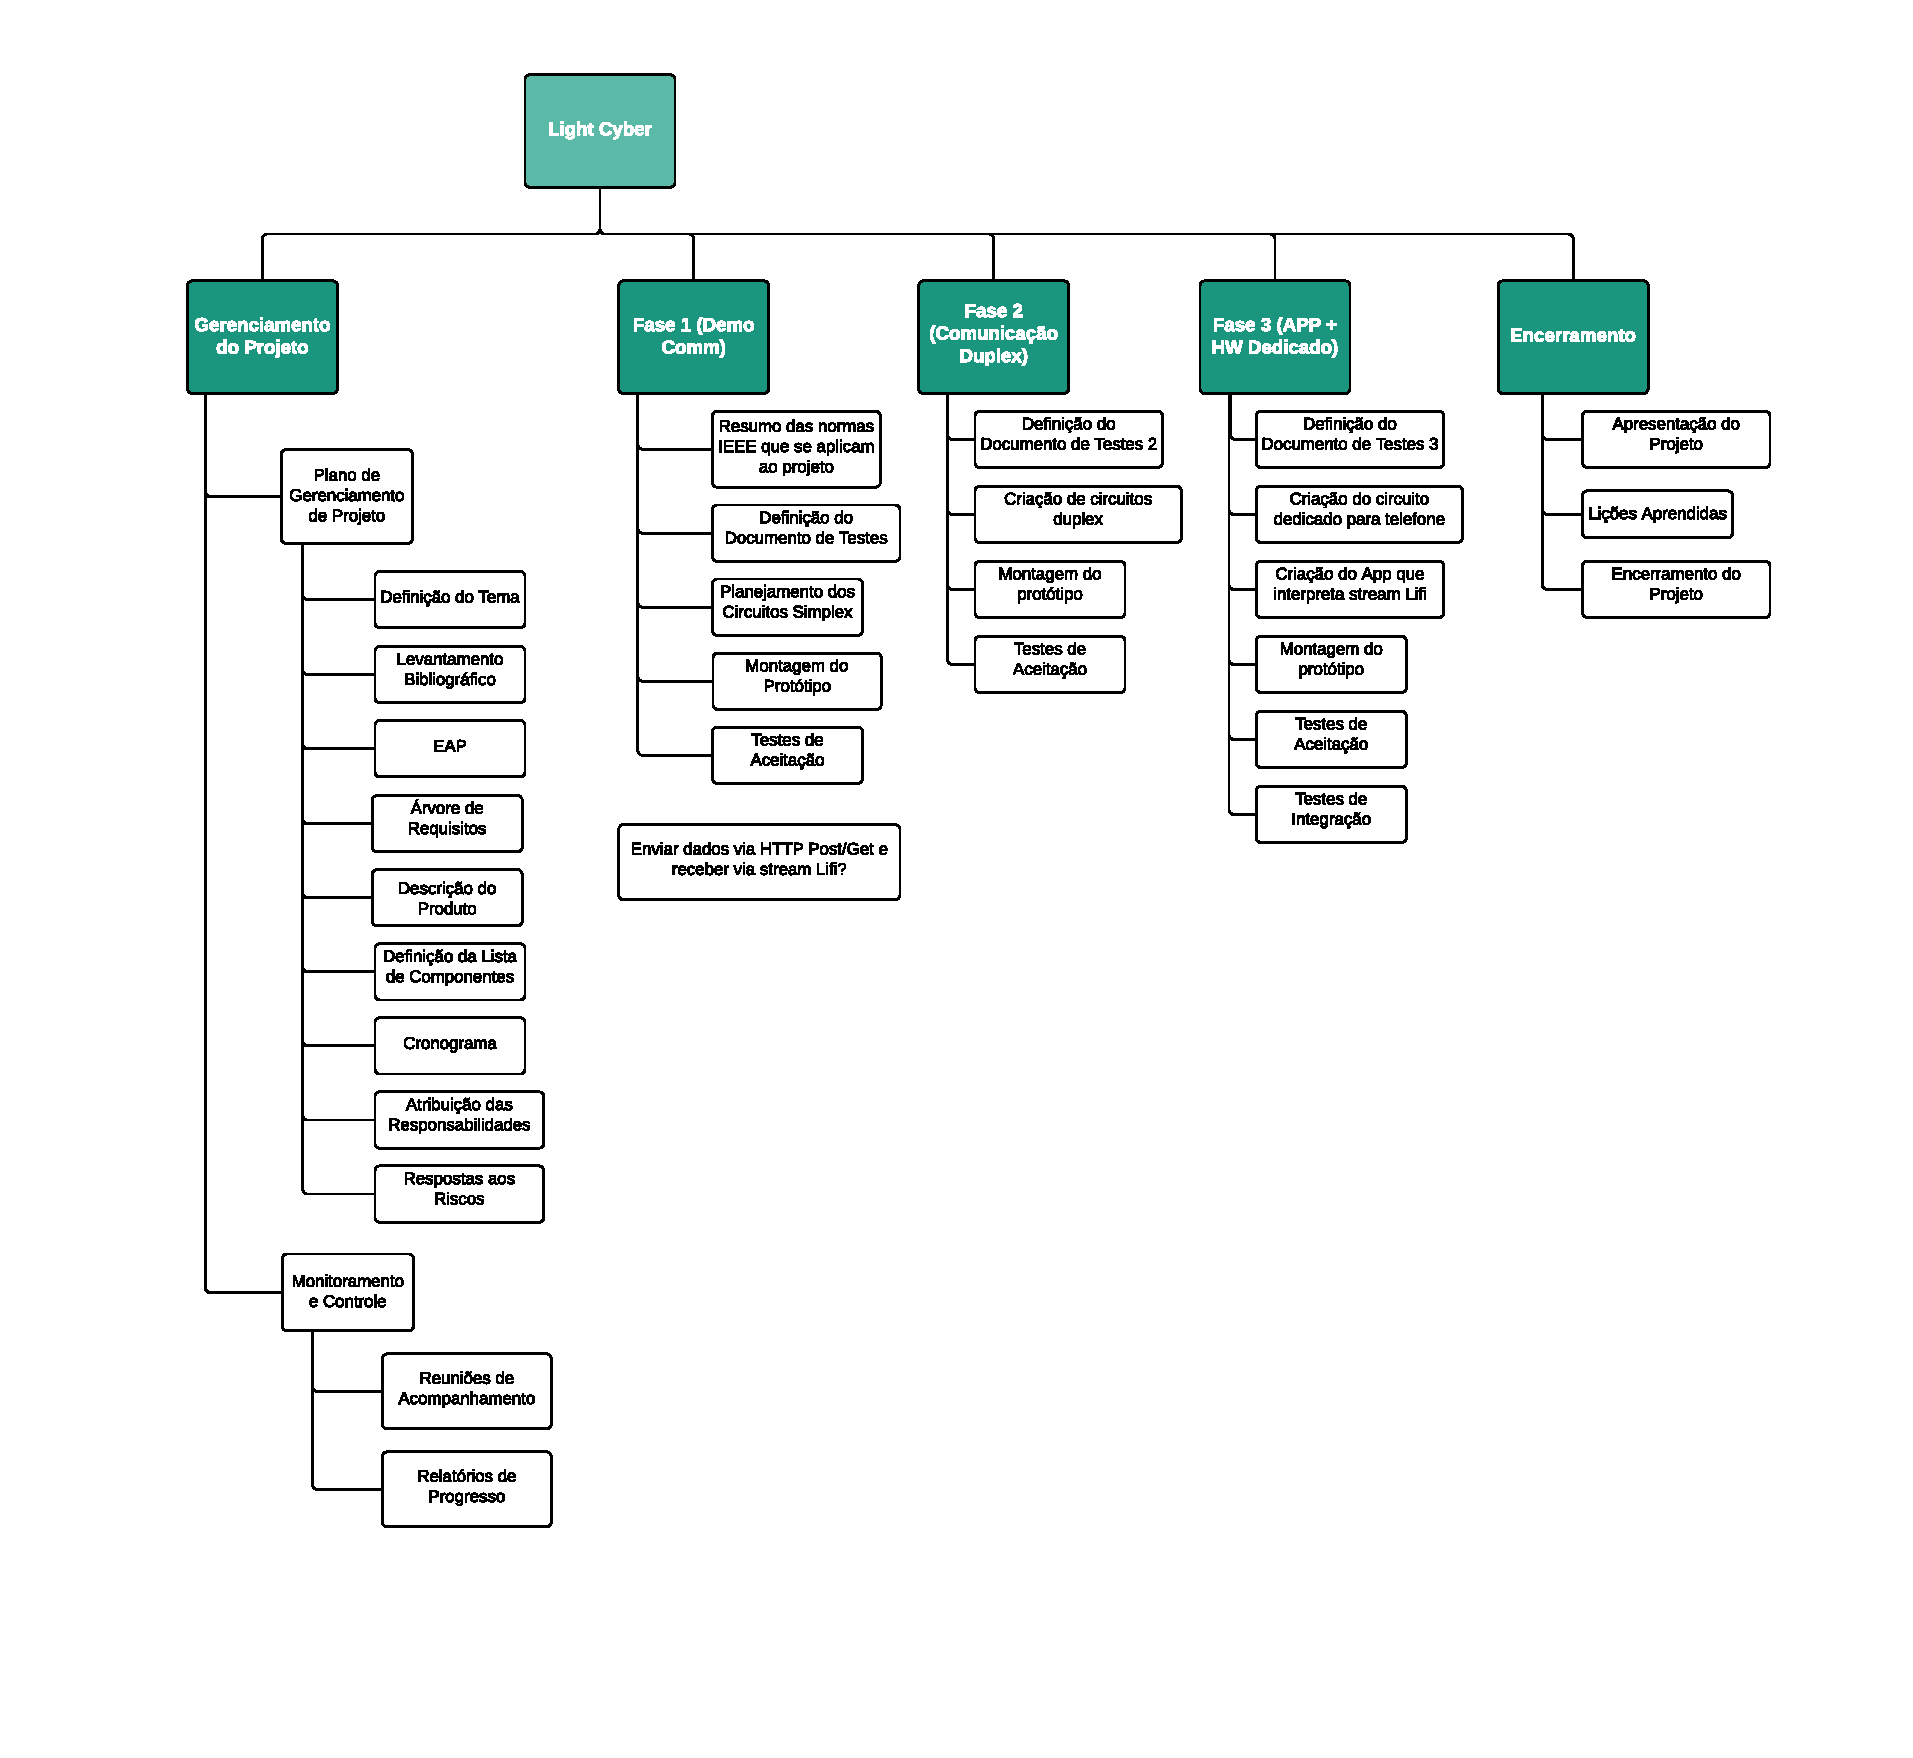
\includegraphics[width=0.8\textwidth, trim={0cm 0cm 0cm 0cm}, clip]{EAP.pdf}
		\legend{Fonte: Autores.}
	\end{figure}

	% ---
	\subsection{Cronograma}\label{subsec-cronograma}
	% ---

	O cronograma do projeto foi planejado a partir dos pacotes de trabalho definidos na Estrutura Analítica de Projeto. Os participantes fizeram reuniões para estimar o tempo de cada um desses pacotes, com a aplicação das estimativas a um calendário, que também considerou as datas de entrega oficiais da disciplina. Com todas as estimativas feitas, a primeira e segunda fases do projeto durariam até o fim de Novembro de 2016, como pode-se observar no diagrama de Gantt na \autoref{fig_gantt}.

	\begin{figure}[h!]
		\caption{\label{fig_gantt}Diagrama de Gantt do projeto LiCy.}
		\centering
		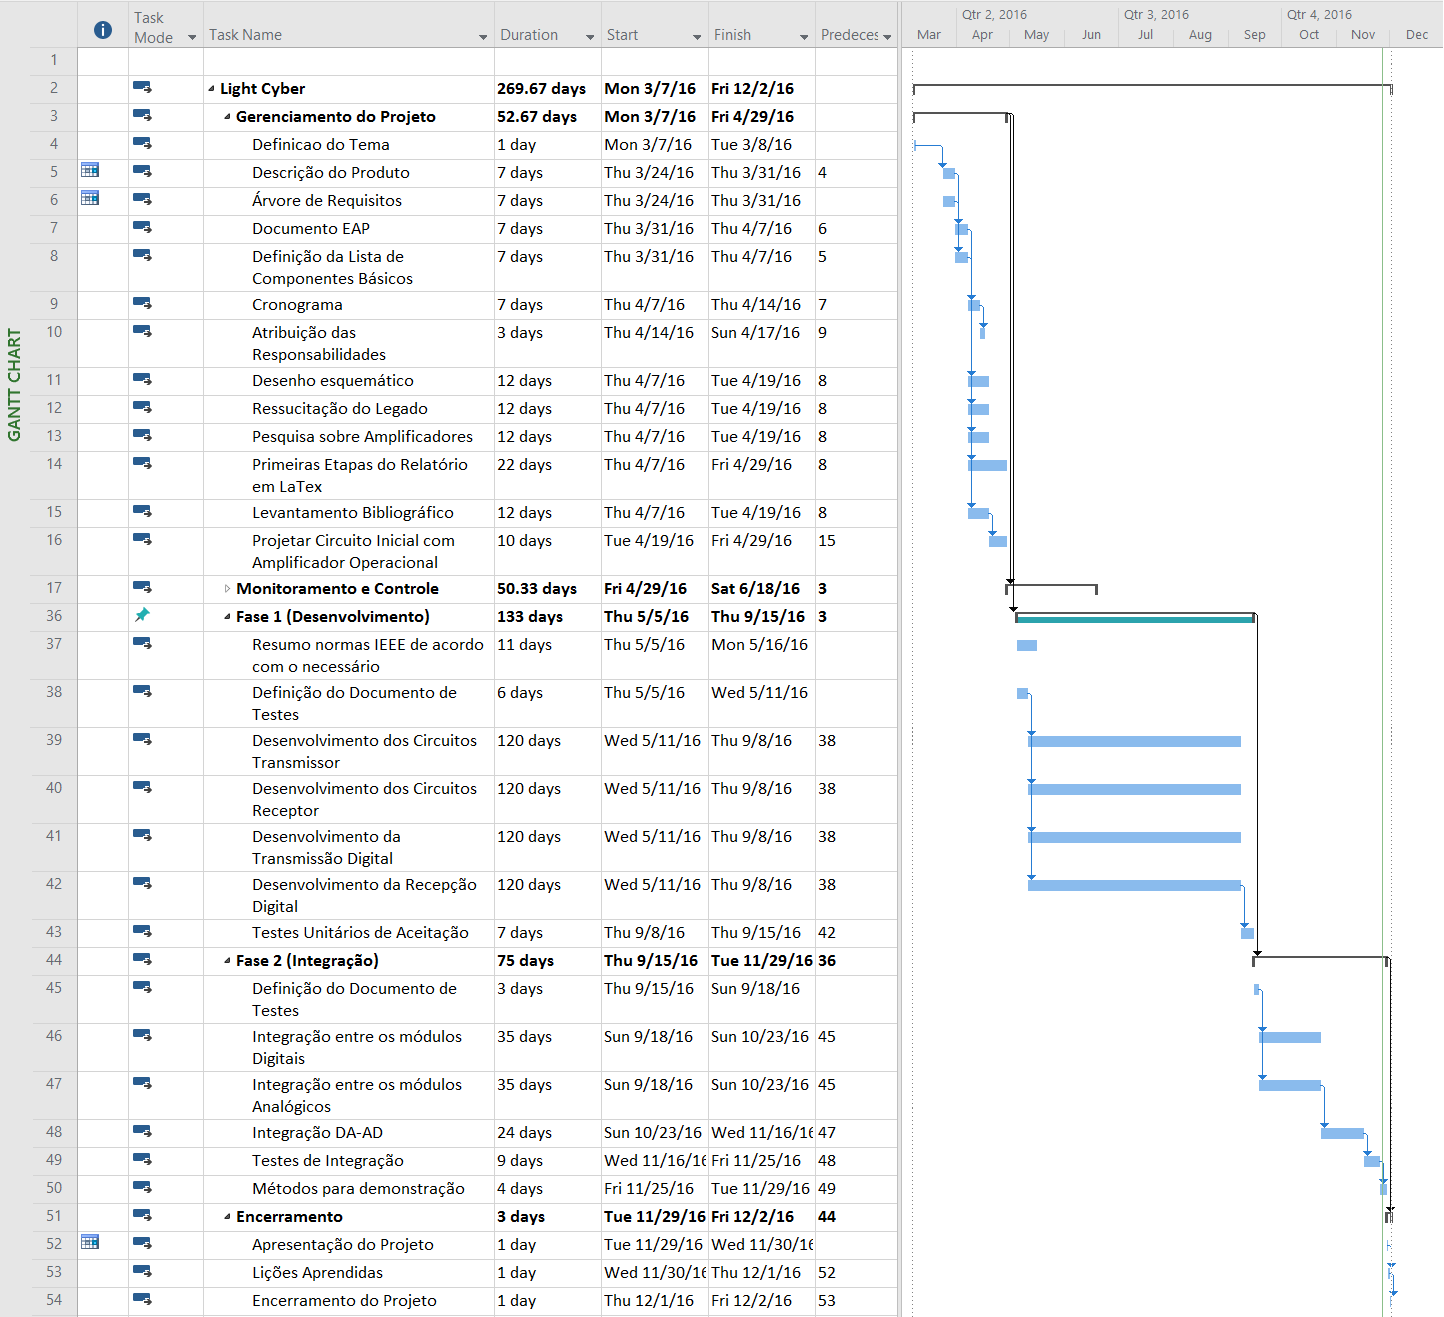
\includegraphics[width=1.0\textwidth]{gantt.png}
		\legend{Fonte: Autores.}
	\end{figure}

	% ---
	\subsection{Requisitos}\label{subsec-requisitos}
	% ---

	Os requisitos foram divididos primeiramente em funcionais e não-funcionais. Além disso, existem outras divisões relacionadas a hardware, estética e módulos do sistema. Para cada requisito foi dado um peso, conforme avaliação da relevância deste requisito para o projeto, de modo que no topo da árvore haja uma soma equivalente a 100.

	% ---
	\subsubsection*{Requisitos Funcionais}\label{subsubsec-requisitos-func}
	% ---

	\paragraph*{Requisitos de hardware digital}

	É importante observar que estes dividem-se entre a lamparina (luminária), que serve de ponto de acesso, e o módulo de recepção, com pesos iguais entre os dois, já que a comunicação é de um para um e ambos têm a mesma importância. Há requisitos em comum entre esses subsistemas, e alguns serão explicados mais à frente. A organização desses requisitos encontra-se abaixo, na \autoref{fig_req1_1}.

	\begin{figure}[h!]
		\caption{\label{fig_req1_1}Requisitos Funcionais de Hardware Digital.}
		\centering
		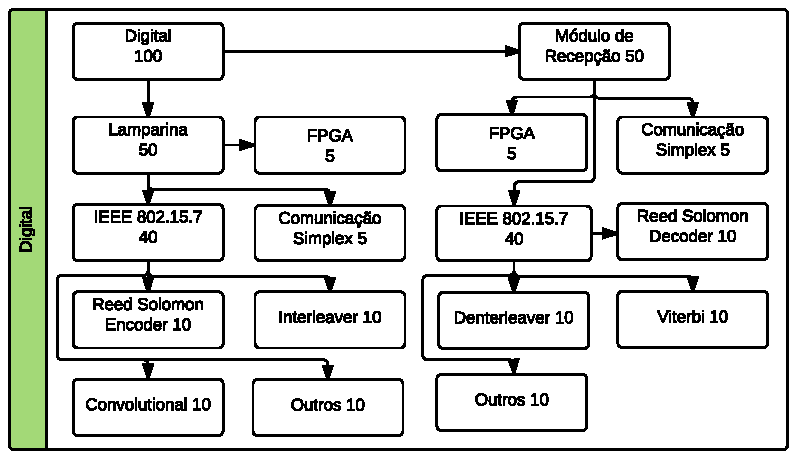
\includegraphics[width=0.5\textwidth]{Req_Tree_Digital.pdf}
		\legend{Fonte: Autores.}
	\end{figure}

	\begin{itemize}
		\item Estar de acordo com a norma IEEE 802.15.7 - que tem o peso mais alto, já que o escopo principal deste trabalho compreende implementá-la;
		\begin{itemize}
			\item Codificador de Reed Solomon. Determinado pela norma, para garantir integridade através da correção de erros;
			\item Entrelaçamento e desentrelaçamento. Métodos que evitam erros em sequências e garantem certo grau de confidencialidade;
			\item Codificação convolucional e decodificador de Viterbi. Ajudam avaliar a chance da mensagem recebida conter erros, aproximando-a da enviada;
			\item Outros requisitos. Dizem respeito a outra parte da codificação definida pela norma, além do pipeline do fluxo de dados e controle, bem como circuitos de sincronismo;
		\end{itemize}
		\item Utilização da FPGA para implementar a camada física. As justificativas para o uso desse componente será apresentada nos próximos itens;
		\item Comunicação simplex um a um, que visa garantir a unilateralidade da comunicação entre dois nós, com recepção e transmissão exclusivas a cada uma das partes.
	\end{itemize}

	A lamparina possui requisitos de hardware próprios, incluindo a habilidade de funcionar como \emph{Access Point}, ou seja, fornecer acesso a uma fonte de dados, que pode ser uma rede local, um computador, a internet, entre outros.

	Já o módulo de recepção tem como requisito de hardware exclusivo a interface com um terminal para se observar os dados recebidos, que é essencialmente um computador ou dispositivo móvel.

	\paragraph*{Requisitos de hardware analógico}
	Dividem-se entre a lamparina e o módulo receptor:

	\begin{figure}[h!]
		\caption{\label{fig_req1_2}Requisitos Funcionais de Hardware Analógico.}
		\centering
		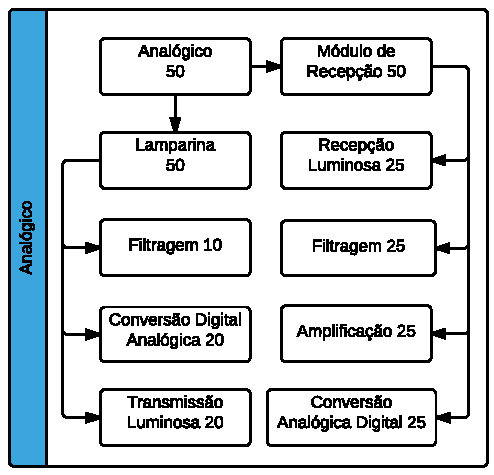
\includegraphics[width=0.5\textwidth]{Req_Tree_Analog.pdf}
		\legend{Fonte: Autores.}
	\end{figure}

	\begin{itemize}
		\item Transmissão e recepção luminosa. Utilizar LED e fotodiodo, para transmitir e receber, respectivamente, os dados modulados através da luz. Adequar a frequência de operação à norma;
		\item Filtragem de sinais. Filtrar a luz ambiente, que é primordial para que a recepção seja bem sucedida, do contrário pode haver muita interferência da luz que não tenha o LED como fonte. Deve fazer com que o sistema se aproxime ao máximo de um cenário ideal, onde há apenas um LED e um fotodiodo num ambiente escuro.
		\item Conversão Digital-Analógica / Analógica-Digital.
	\end{itemize}


	\subsubsection*{Requisitos Não-Funcionais}\label{subsubsec-requisitos-nfunc}

	Foram especificados através da seguinte estrutura:

	\begin{figure}[h!]
		\caption{\label{fig_req2}Requisitos Não Funcionais.}
		\centering
		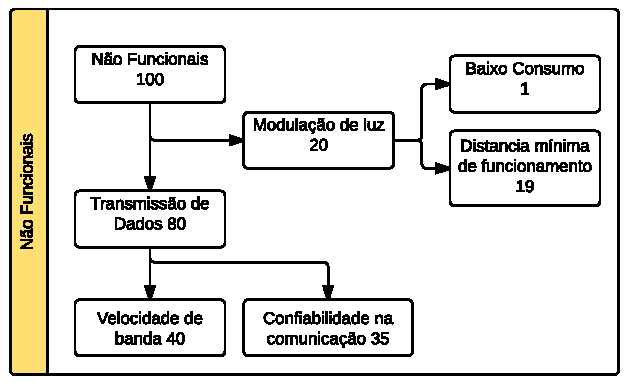
\includegraphics[width=0.5\textwidth]{Req_Tree_NFunc.pdf}
		\legend{Fonte: Autores.}
	\end{figure}

	\paragraph*{Transmissão de dados}
	Uma das principais preocupações é manter a velocidade da banda conforme a especificação da norma IEEE 802.15.7 para cada camada física (PHY) correspondente. É também primordial garantir a confiabilidade na comunicação, de modo que se possa garantir que os \textit{bits} recebidos estão corretos e quando possível e necessário, corrigí-los, observando as limitações que serão discutidas posteriormente no que diz respeito à norma (ver módulos de codificação e decodificação).

	\paragraph*{Modulação de luz}
	O requisito mais importante é garantir o funcionamento do sistema a uma distância de até 1 metro, considerando uma aplicação residencial do produto. Secundariamente, há o requisito de manter um baixo consumo de energia, que apesar de fundamental em produtos de tecnologia da informação, foge do escopo deste estudo.

	% ---
	\section{Norma IEEE 802.15.7}\label{sec-norma}
	% ---
	\begin{figure}[htb]
		\caption{\label{fig_architecture}Arquitetura de dispositivos VPAN.}
		\centering
		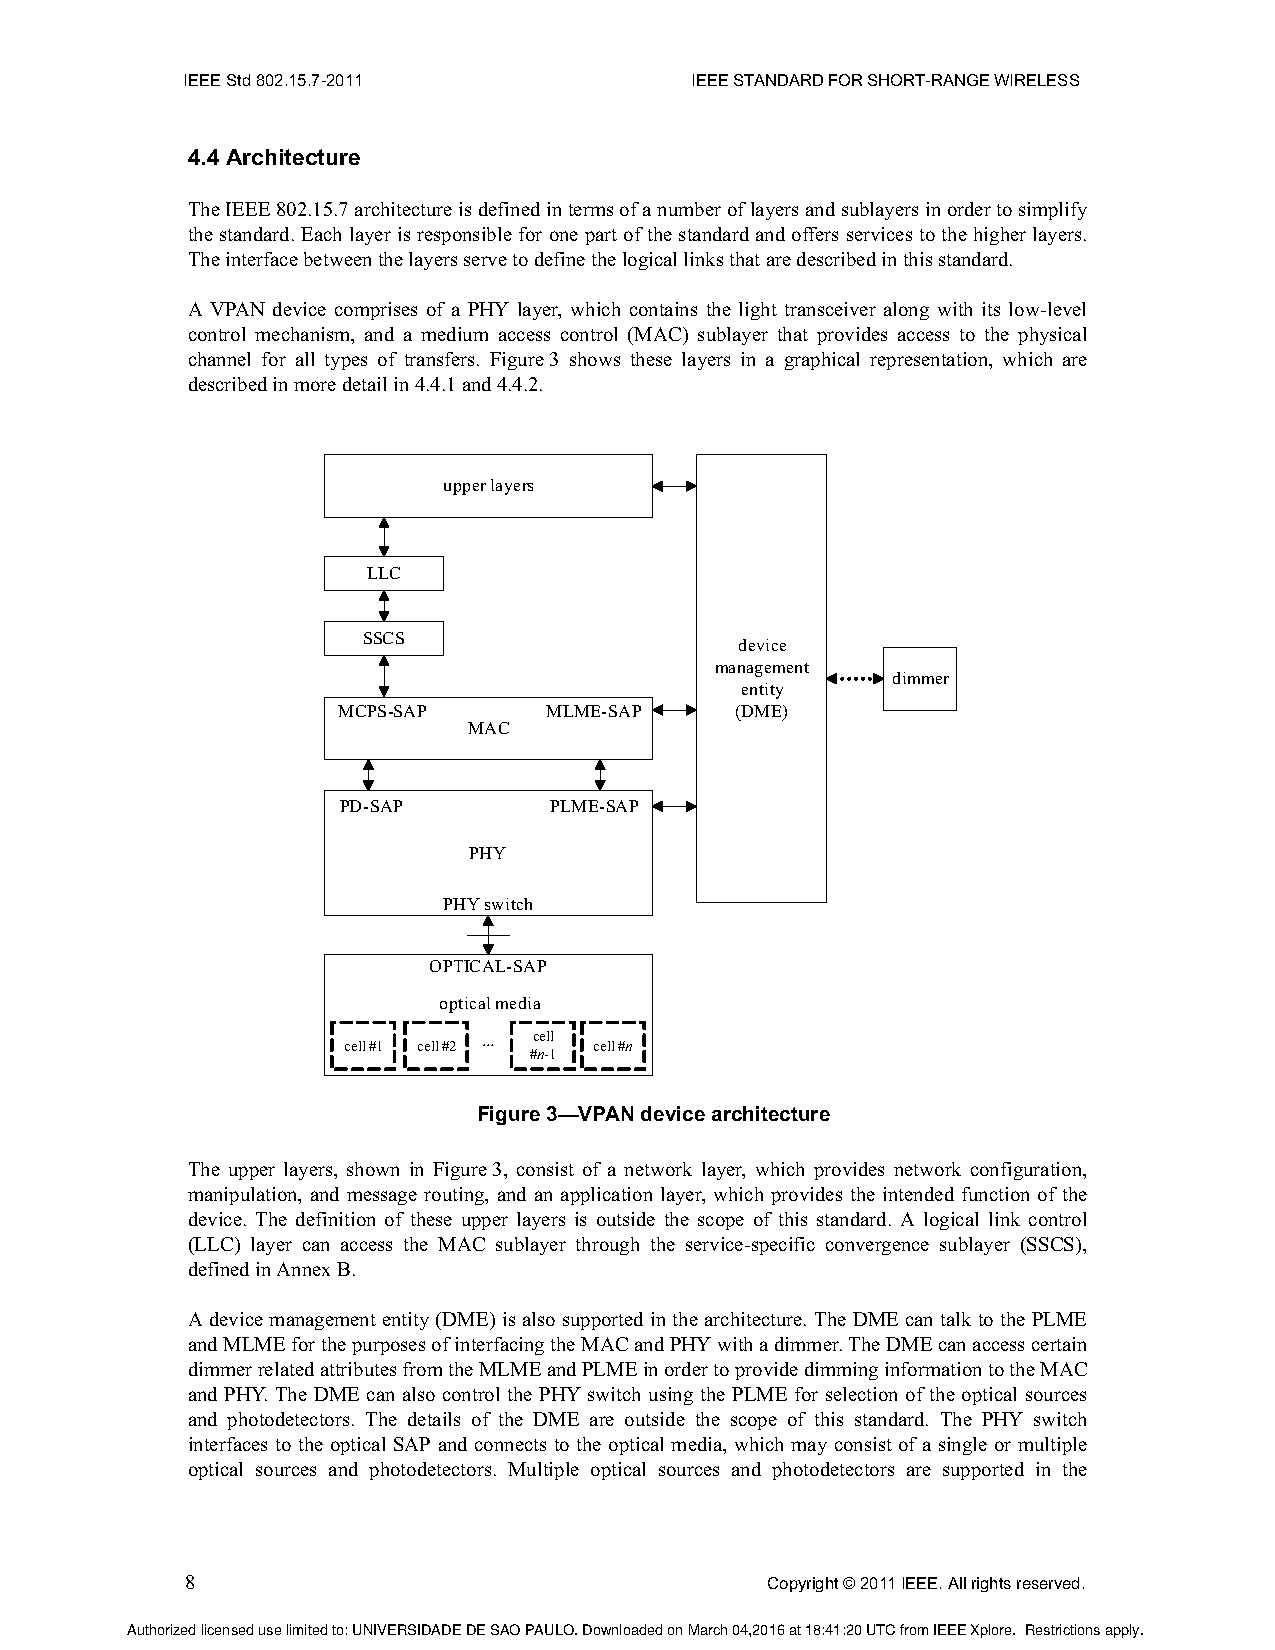
\includegraphics[width=0.5\textheight,trim={5cm 9.6cm 5.3cm 7cm}, clip]{pag31.pdf}
		\legend{Fonte: IEEE 802.15.7}
	\end{figure}

	A norma 802.15.7 estabelece um padrão para comunicação via luz, abarcando definição de topologias de rede, codificação da informação, divisão das camadas da arquitetura do sistema de comunicação, ordem e conteúdo de cabeçalhos para cada camada e definições sobre a segurança do \textit{link}. A arquitetura de um sistema LiFi completo está definida na \autoref{fig_architecture}.
	O trabalho focará no estudo e implementação da camada PHY. Os modos de operação da subcamada PHY I estão listado na \autoref{tab_phy1}.

	\begin{table}[h!]
		\caption{\label{tab_phy1}Modos de operação da camada PHY I de Li-Fi.}
		\centering
		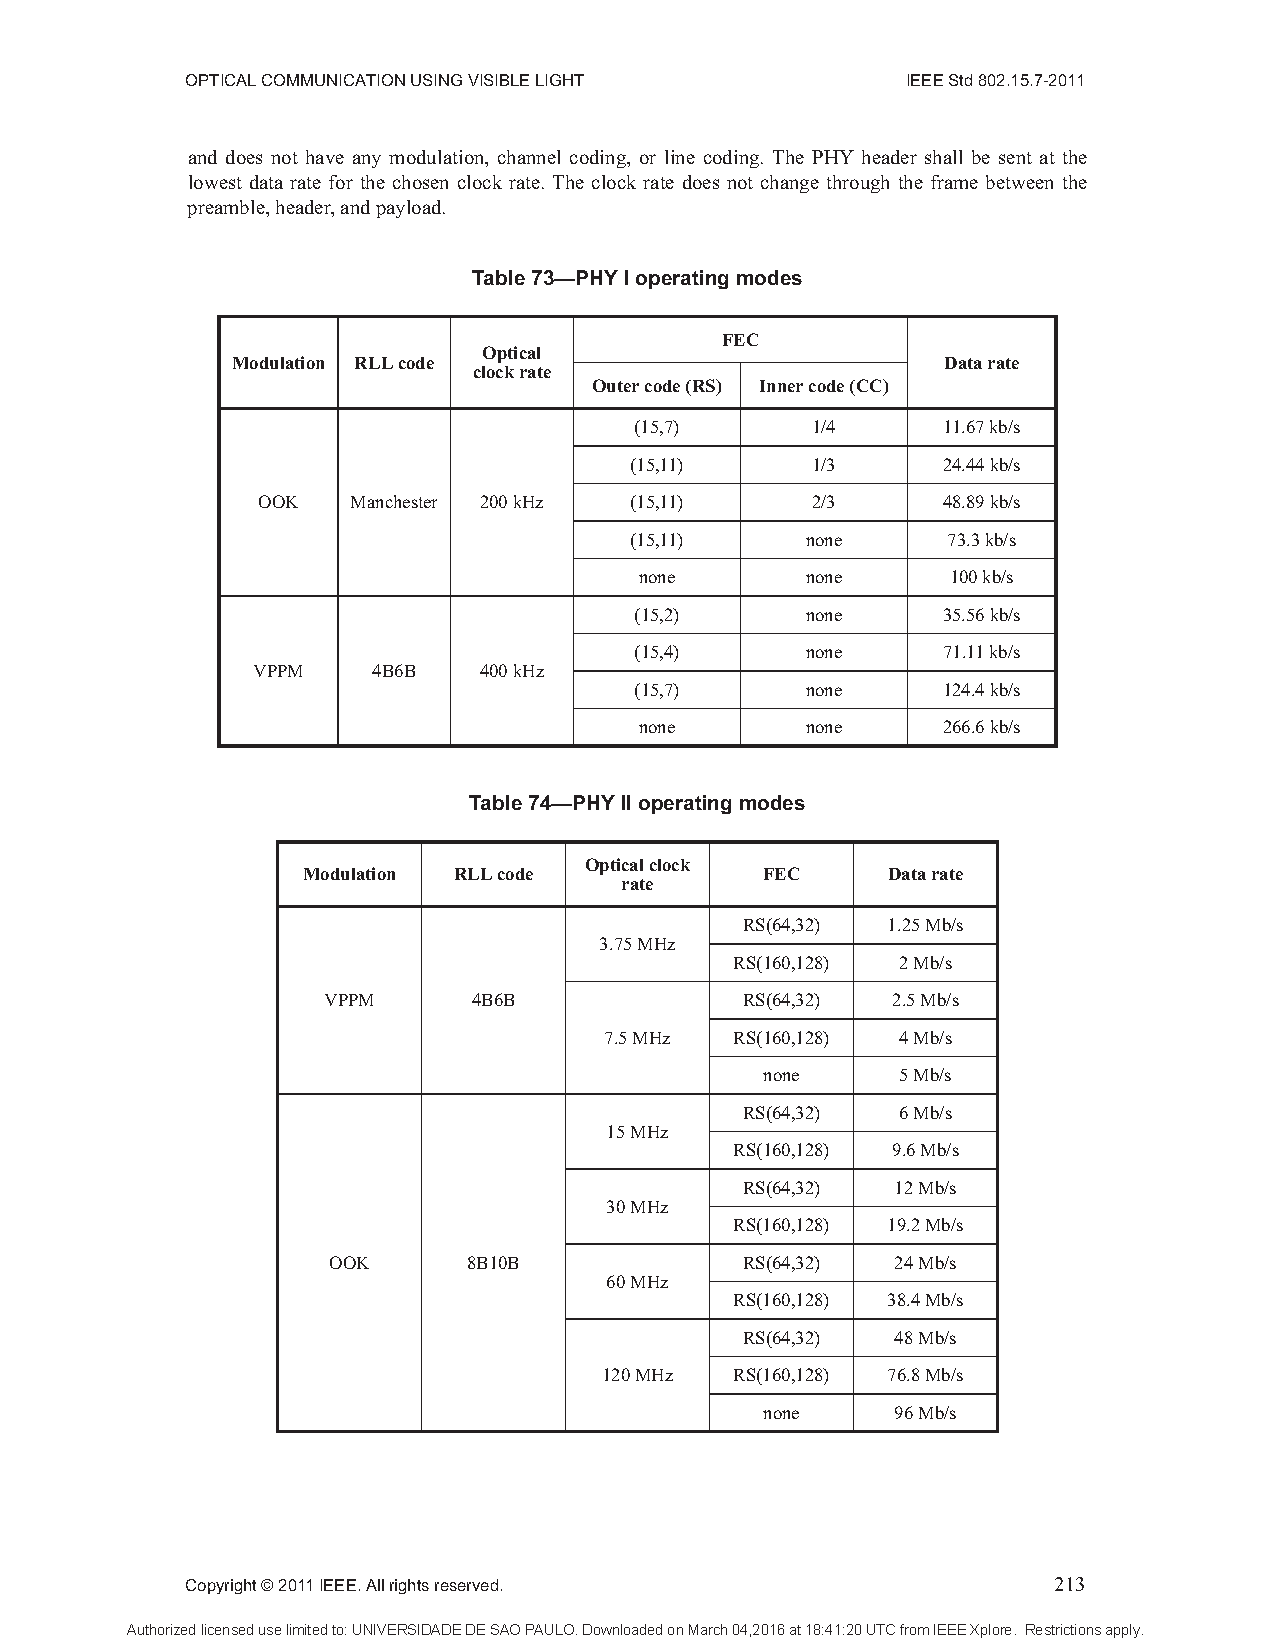
\includegraphics[clip, trim=37mm 151mm 36mm 51mm,  width=0.7\textwidth]{pag213.pdf}
		\legend{Fonte: IEEE 802.15.7}
	\end{table}

	\subsection{Transmissão}

	Nessa seção será discutido o processo de transmissão de dados via luz, levando em conta a norma.
	% Repetido abaixo códigos cíclicos de correção de erro, redução de erros em \emph{burst} e protocolos RLL, especificados pela norma IEEE. Para realizar a transmissão, é necessário passar pelas etapas do diagrama abaixo:

		\begin{figure}[htb]
			\caption{\label{fig_transmission_phy1}Diagrama de blocos da codificação da mensagem.}
			\centering
			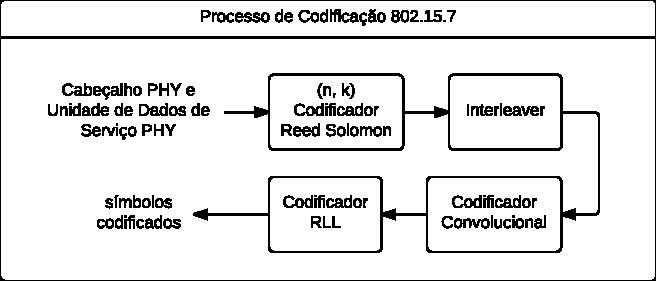
\includegraphics[width=0.4\textheight]{PHY1-transmission.pdf}
			\legend{Fonte: Autores.}
		\end{figure}

	Para que os dados transmitidos sejam recebidos corretamente, a norma estabelece algumas regras para codificação da mensagem, a fim de garantir recuperação de erros, redução de erros em \emph{burst}, facilidade na sincronia do \textit{clock}, entre outros detalhes. A \autoref{fig_transmission_phy1} ilustra os passos necessários para compor a mensagem antes de sua transmissão. Esses passos estarão detalhados nas seções a seguir.


	\subsubsection*{Codificação Reed Solomon}

	Com o intuito de adicionar redundância de informação na mensagem, a norma estabelece um mecanismo de correção de erros antecipada (FEC). Mais especificamente, o código de Reed Solomon, apresentado originalmente em \cite{reed-solomon-original} e também discutido em \cite{rs-bbc}.

	Os códigos Reed Solomon são compostos por símbolos de mais de um \textit{bit}. O número de erros é considerado como sendo o total de símbolos com pelo menos um \textit{bit} com erro. Isso o torna efetivo para corrigir erros em rajadas, já que uma sequência de \textit{bits} errados dentro de um mesmo símbolo é considerada como apenas um erro.

	Os principais parâmetros de um código Reed Solomon são $(n, k)$, onde $n$ é o número de símbolos de um bloco de código e $k$ é o tamanho da mensagem em número de símbolos. Portanto, o bloco terá $n - k$ símbolos de paridade, usualmente designados como $2t$, sendo que a capacidade de correção é de até $t$ símbolos.

	\paragraph*{Corpos de Galois}

	A codificação e decodificação de Reed Solomon usam em seus algoritmos operações aritméticas de multiplicação e adição de corpos finitos. A norma IEEE 802.15.7 define que para a camada PHY 1, usa-se Galois Fields 16, ou na notação corrente na literatura: GF(16). Um corpo de Galois é um conjunto de $2m - 1$ elementos, cada qual representado por um polinômio de grau $m - 1$, com coeficientes binários. Em suma, um elemento de GF(16) pode ser representado a partir de símbolos de 4 \textit{bits}, totalizando 16 elementos de 0000 a 1111.

	A adição e subtração de dois corpos de Galois é dada pela soma ou subtração dos coeficientes de dois polinômios. Além disso as operações são feitas \textit{bit} a \textit{bit}, sem que haja \textit{bits} de ``vai um'' para coeficientes subsequentes. Caso os dois coeficientes tenham o mesmo valor, que pode ser 1 ou 0, o resultado da sua soma ou subtração deve ser 0. Caso contrário, a soma equivale a 1, de maneira que essa operação é perfeitamente representável pela função lógica de OU exclusivo, tanto para adição como subtração.

	Os corpos de Galois são definidos com base no gerador polinomial de corpos, que é um polinômio irredutível, de grau $m$. Para GF(16) existe por exemplo, esta opção:
	\begin{equation}
	p(x) = x^{4} + x + 1
	\end{equation}
	A norma IEEE 802.7.15 não especifica qual gerador polinomial deve ser usado, portanto neste estudo foi usada a opção do exemplo. O processo de geração neste caso resulta nos elementos finitos da Tabela~\ref{tab:galois}.
	\begin{table}[]
		\centering
		\caption{Corpos de Galois (16)}
		\label{tab:galois}
		\begin{tabular}{|c|c|}
			\hline
			Elemento & Representação binária \\ \hline
			$\alpha^{0}$   & 0001                  \\ \hline
			$\alpha^{1}$   & 0010                  \\ \hline
			$\alpha^{2}$   & 0100                  \\ \hline
			$\alpha^{3}$   & 1000                  \\ \hline
			$\alpha^{4}$   & 0011                  \\ \hline
			$\alpha^{5}$   & 0110                  \\ \hline
			$\alpha^{6}$   & 1100                  \\ \hline
			$\alpha^{7}$   & 1011                  \\ \hline
			$\alpha^{8}$   & 0101                  \\ \hline
			$\alpha^{9}$   & 1010                  \\ \hline
			$\alpha^{10}$  & 0111                  \\ \hline
			$\alpha^{11}$  & 1110                  \\ \hline
			$\alpha^{12}$  & 1111                  \\ \hline
			$\alpha^{13}$  & 1101                  \\ \hline
			$\alpha^{14}$  & 1001                  \\ \hline
			$\alpha^{15}$  & 0000                  \\ \hline
		\end{tabular}
	\end{table}

	A multiplicação entre dois corpos de Galois ocorre, em termos de aritmética comum, pela multiplicação de dois polinômios, seguida da divisão pelo gerador polinomial. Já a divisão  de corpos finitos pode ser feita através da operação de inversão do divisor e multiplicação desse resultado pelo dividendo, seguindo os passos indicados anteriormente para a multiplicação.

	\paragraph*{Codificação}

	Para gerar um código de Reed Solomon a partir dos corpos finitos, é necessário um polinômio gerador de código. Este polinômio possui $2t$ fatores, de maneira que o grau do polinômio representado por $C(x)$ (bloco codificado, com grau $n$) seja a soma do grau de $M(x)$ (a própria mensagem dentro do bloco codificado, com grau $k$) e $G(x)$ (polinômio codificador, com grau $2t = n - k$). O polinômio gerador de código deve ter a seguinte forma:

	\begin{equation}
	g(x) = (x + \alpha^{i})(x + \alpha^{i+1})...(x + \alpha^{i + 2t - 1})
	\end{equation}

	As raízes são escolhidas como corpos finitos de Galois consecutivos. Para esse estudo, usaram-se como raízes os elementos consecutivos de $\alpha^{0}$ a $\alpha^{7}$. Por exemplo, para um código (15, 7), usado posteriormente neste projeto:

	\begin{equation}
	g(x) = (x + \alpha^{0})(x + \alpha^{1})(x + \alpha^{2})(x + \alpha^{3})(x + \alpha^{4})(x + \alpha^{5})(x + \alpha^{6})(x + \alpha^{7})
	\end{equation}

	\begin{equation}
	g(x) = \alpha^{13}x^{7} + \alpha^{0}x^{6} + \alpha^{1}x^{5} + \alpha^{13}x^{4} + \alpha^{8}x^{3} + \alpha^{14}x^{2} + \alpha^{4}x + \alpha^{13}
	\end{equation}

	Neste caso, a mensagem $M(x)$ é codificada da seguinte maneira:

	\begin{equation}
	\frac{M(x)x^{n-k}}{G(x)} = q(x) + \frac{r(x)}{g(x)}
	\end{equation}

	Desta forma, são produzidos um quociente $q(x)$ e um resto $r(x)$. Por manipulação algébrica, temos que o bloco codificado pode ser representado da seguinte forma:

	\begin{equation}
	M(x)x^{n-k} + r(x) = g(x)q(x)
	\end{equation}

	Portanto, o bloco codificado $C(x)$ é composto por $M(x)$ deslocada, somada a $r(x)$, na prática equivalendo à \autoref{fig_reed_solomon_message}, com os símbolos de dados transmitidos em esquema de fila, seguidos dos símbolos de paridade.

	\begin{figure}[!htb]
		\caption{\label{fig_reed_solomon_message}Diagrama de blocos da codificação da mensagem.}
		\centering
		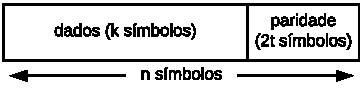
\includegraphics[width=0.4\textheight]{frame/rs-codeword.pdf}
		\legend{Fonte: Autores.}
	\end{figure}

	Finalmente, a representação do codificador de Reed Solomon (15, 7) em hardware equivale a mostrada na \autoref{fig:reedsolomon}.

	\begin{figure}[!htb]
		\caption{\label{RS_encoder_logic}Circuito lógico de codificação Reed Solomon (15,7).}
		\centering
		\includegraphics[width=0.6\textheight]{RS_Encoder.png}
		\legend{Fonte: Autores.}
		\label{fig:reedsolomon}
	\end{figure}

	É possível observar nos registradores e multiplicadores de Galois a estrutura de um polinômio e seus índices. A mensagem a que se vai adicionar redundância deve passar pela ``entrada'', com um ciclo de \textit{clock} para cada símbolo, levando portanto 7 ciclos para finalizar o cálculo das paridades para um código (15, 7). Os 8 símbolos de paridade devem então serem passados através de registradores de deslocamento, com a mudança do sinal de seleção, de maneira também a zerar a saída da porta lógica AND à direita. Sendo assim, os valores dos registradores não são afetados pelos somadores, já que as operações de multiplicação e soma de Galois estarão recebendo uma das entradas igual a 0000. Em suma, o processo de codificação leva tantos ciclos quantos forem os símbolos do bloco codificado, ou o valor denotado por $n$.

	\subsubsection*{Interleaver}

	O processo de entrelaçamento é utilizado para aprimorar a performance de mecanismos de correção de erros antecipados. Ele se baseia no fato de que canais de comunicação não são estocásticos, então erros ocorrem em sequência e não independentemente.

	O entrelaçamento serve para distribuir os dados de forma que erros em rajadas serão distribuídos em múltiplas palavras de código, facilitando o processo de recuperação de erros.

	Para melhor demonstrar a aplicação do entrelaçador, serão exemplificadas várias situações utilizando um sistema de recuperação de erros em um canal com ruídos (que costumam ser \textit{bit-flip}). Na primeira, não é aplicado o entrelaçamento e a mensagem é recuperável com redundância.

	\begin{verbatim}
	    Burst = 2, Redundância = 3, Sem entrelaçamento
	    Mensagem inicial:                             abcdefg
	    Mensagem com redundância:                     aaabbbcccdddeeefffggg
	    Transmissão com erros em burst:               aaabbbc__dddeeefffggg
	    Mensagem recuperada:                          abcdefg
	\end{verbatim}

	Mesmo após dois caracteres perdidos em sequência, foi possível recuperar as perdas do canal. Isso ocorreu porque o \textit{burst} do erro foi menor que sua capacidade de recuperação. Na situação a seguir, novamente sem entrelaçamento, a mensagem não é recuperável com redundância.

	\begin{verbatim}
	    Burst = 4, Redundância = 3, Sem entrelaçamento
	    Mensagem inicial:                             abcdefg
	    Mensagem com redundância:                     aaabbbcccdddeeefffggg
	    Transmissão com erros em burst:               aaabbbcc____eeefffggg
	    Mensagem recuperada:                          abc_efg
	\end{verbatim}

	Mesmo com a redundância aplicada, a informação \textit{d} foi perdida devido a erros em \textit{burst}. Aplicando entrelaçamento, a mesma mensagem pode ser recuperada facilmente, a seguir:

	\begin{verbatim}
	    Burst = 4, Redundância = 3, Com entrelaçamento
	    Mensagem inicial:                             abcdefg
	    Mensagem com redundância:                     aaabbbcccdddeeefffggg
	    Interleaving:                                 abcdefgabcdefgabcdefg
	    Transmissão com erros em sequência:           abcdefgab____gabcdefg
	    Deinterleaving:                               aaabbbc_cd_de_ef_fggg
	    Mensagem recuperada:                          abcdefg
	\end{verbatim}

	A mensagem recebida foi recuperada porque os erros foram distribuídos em partes diferentes da mensagem, que foi entrelaçada. Os dados resultantes puderam ser inferidos pela redundância aplicada.

	\subsubsection*{Puncture}

	O módulo de punção é utilizado para reduzir o \textit{overhead} do \textit{padding}, e é aplicado depois do \textit{interleaver}. A função da punção é remover alguns bits de paridade da sequência, e equivale a utilizar um algoritmo de correção de erros com menos redundância. Neste caso, visa os bits de \textit{padding}, que não representam informação e são colocados apenas para completar o pacote até que o tamanho seja uma potência de dois. O efeito é uma redução na taxa do código, que será explicada nas seções subsequentes.

	\subsubsection*{Código Convolutional}

	O módulo de código convolucional é um código de correção de erros que converte a mensagem em símbolos de paridade. Ele se utiliza de uma janela deslizante para receber e armazenar uma parte dos dados de entrada. Alguns subgrupos de \textit{bits} dentro da janela, definidos pelos geradores polinomiais, são utilizados para gerar os \textit{bits} de paridade. A operação de \textit{exclusive or} entre os \textit{bits} de um subgrupo gera um \textit{bit} de paridade. A norma define os parâmetros do código na \autoref{table:convolutional-params} de acordo com a camada PHY I.

	\begin{table}[ht]
		\caption{Parâmetros do Código Convolucional da camada PHY I.}
		\centering
		\begin{tabular}{c c c}
			\hline
			Parâmetro & Valor & Descrição \\ \hline
			K & 7 & comprimento da janela deslizante \\
			R & 1/4 & taxa de \textit{bits} / paridade \\
			G & $g_{0} = 133_{8}$; $g_{1} = 171_{8}$; $g_{2} = 165_{8}$ & polinômio gerador \\ \hline
		\end{tabular}
		\label{table:convolutional-params}
		\legend{Fonte: Autores.}
	\end{table}

	No documento da norma há uma figura que especifica a implementação do codificador. Estudando-a em detalhes, foram encontrados erros na figura, pois os \textit{bits} utilizados para gerar as paridades eram extraídos de geradores polinomiais errados. A \autoref{figure:convolutional-schematics} esquematiza um codificador com os polinômios corrigidos. A cada \textit{bit} $X_{n}$ de entrada, o código convolucional gera três paridades: $A_{0}$, $B_{0}$ e $C_{0}$, por isso 1/3.
	\begin{figure}[h!]
		\caption{\label{figure:convolutional-schematics}Esquemático do Codificador Convolucional com taxa 1/3, os quadrados representam registradores e os retângulos os somadores.}
		\centering
		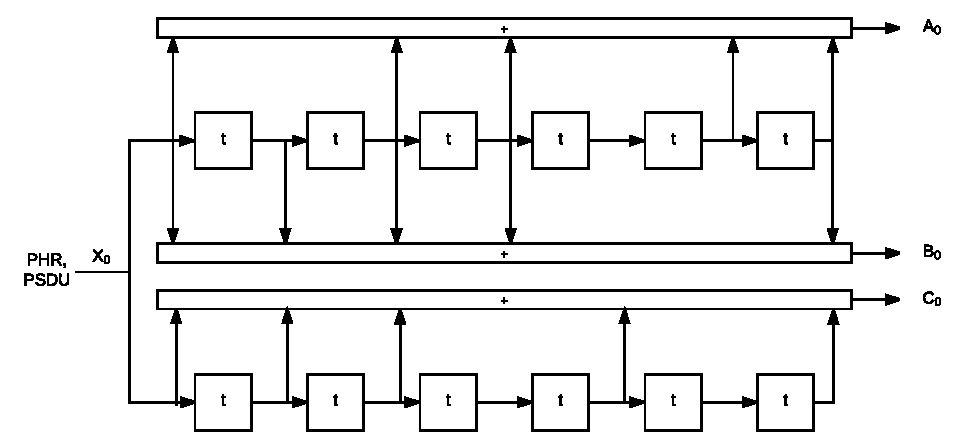
\includegraphics[width=0.5\textheight]{convolutional/schematics.pdf}
		\legend{Fonte: Autores}
	\end{figure}


	Nota-se que o codificador especificado pela norma tem taxa 1/3, e não de 1/4, como especificado na norma. Para obter uma taxa de 1/4 deve-se realizar operação de \textit{puncture} no código de taxa 1/3 para um de taxa 1/2, como mostrado na \autoref{figure:convolutional-puncture}, e depois usando um código de repetição como na \autoref{figure:convolutional-repetition}.

	\begin{figure}[h!]
		\caption{\label{figure:convolutional-puncture}Padrão de \textit{puncture} para obter código a taxa 1/2.}
		\centering
		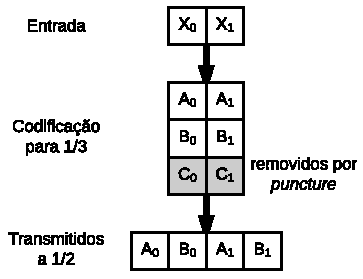
\includegraphics[width=0.25\textheight]{convolutional/puncture.pdf}
		\legend{Fonte: Autores.}
	\end{figure}
	\begin{figure}[h!]
		\caption{\label{figure:convolutional-repetition}Padrão de repetição utilizado para obter um código com taxa 1/4.}
		\centering
		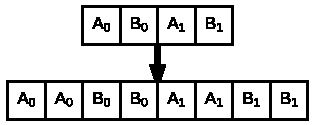
\includegraphics[width=0.25\textheight]{convolutional/repetition.pdf}
		\legend{Fonte: Autores.}
	\end{figure}

	Como a saída do codificador é serial de um \textit{bit}, observa-se que esse código cria um \textit{overhead} na velocidade da transmissão da mensagem. Os \textit{bits} entram no codificador convolucional a uma taxa de t \textit{bits}/tempo e saem a uma taxa de t/4 \textit{bits}/tempo.

	\subsubsection*{Codificação RLL}

	Para a primeira camada de implementação PHY I, será escolhida a codificação RLL Manchester. A codificação Manchester divide o \textit{bit} do dado ao meio, de maneira que a primeira metade deve obrigatoriamente assumir um valor diferente da segunda metade. Em outras palavras, caso a entrada a ser codificada seja 0 por um tempo $2t$, a saída deve ser 01, com cada \textit{bit} com tempo $t$ de transmissão como se verifica na \autoref{tabela_cod_manchester}. Analogamente, caso o \textit{bit} de entrada seja 1, a saída deve ser 10.
	\begin{table}[ht]
		\caption{Codificação Manchester.}
		\centering
		\begin{tabular}{c c}
			\hline
			\textit{bit} & \textit{manchester symbol} \\ \hline
			0 & 01 \\
			1 & 10 \\ \hline
		\end{tabular}
		\label{tabela_cod_manchester}
		\legend{Fonte: Tabela 103 da norma 802.15.7}
	\end{table}
	Uma maneira prática de se obter um codificador Manchester é através da aplicação da operação de OU exclusivo, ou XOR em dois sinais de entrada. Um destes sinais é a própria mensagem a ser codificada, o outro sinal deve ser um \textit{clock} com o dobro da frequência da mensagem. É importante observar que para essa codificação ser eficiente, os dois sinais devem estar sincronizados, de maneira que um período de \textit{clock} seja exatamente equivalente à duração do bit da mensagem de entrada.

	\subsection{Recepção}\label{section_norma_recepcao}

	Após a codificação dos dados, é necessário realizar a sua decodificação. Esse processo inclui a reversão dos processos de codificação e correção de erros, caso existam e seja possível corrigir. No entanto isso não é trivial, pois a norma não especificou nenhum algoritmo para decodificar nem corrigir erros. Foi necessário realizar uma pesquisa para descobrir os métodos mais adequados para decodificação de cada etapa, que estão esquematizadas na \autoref{fig_reception_phy1}. Esses algoritmos estão descritos em detalhes abaixo.

	\begin{figure}[!htb]
		\caption{\label{fig_reception_phy1}Diagrama de blocos da decodificação da mensagem.}
		\centering
		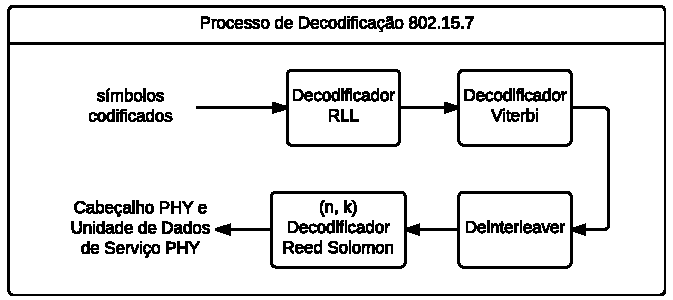
\includegraphics[width=0.4\textheight]{PHY1-reception.pdf}
		\legend{Fonte: Autores.}
	\end{figure}

	\subsubsection*{Decodificação RLL}

	A decodificação do código Manchester ocorre da mesma forma que a codificação, porém com um sinal de \textit{clock} cuja frequência é idêntica à do \textit{clock} de codificação. Portanto, o período do \textit{clock} deve ser o dobro do tempo de duração do \textit{bit} da mensagem. Uma consequência dessa definição é que os dados transmitidos entre um codificador e um decodificador Manchester têm o dobro da frequência da mensagem original, embora a frequência com que os dados efetivos são transmitidos seja a mesma.

	A identificação de erros pode acontecer de diversas formas. É possível, por exemplo, criar uma máquina de estados que identifique a entrada de três \textit{bits} idênticos consecutivos, o que sinaliza erro no caso do código de Manchester. Um dos motivos para esse erro pode ser um código deslocado em até metade de um ciclo do \textit{clock} da entrada do decodificador, e neste caso pode-se corrigir o erro através de uma correção simples, como um \textit{shift register}. Caso o número de \textit{bits} idênticos consecutivos seja superior a dois, a correção do erro se torna muito mais trabalhosa, motivo pelo qual esse tipo de correção não foi abordado neste estudo.

	\subsubsection*{Decodificação Viterbi}\label{section:method-viterbi}

	A seção a seguir explica os conceitos fundamentais para o entendimento do decodificador Viterbi: máquinas de estado, tabela Trellis, o algoritmo de decodificação \textit{Viterbi} e sua simplificação \textit{Fangled} Viterbi.

	\paragraph*{Máquina de Estados}

	A visão de máquinas de estado é uma maneira elegante de explicar o funcionamento do transmissor (e do receptor) e é explicada a seguir. O transmissor começa no estado inicial (marcado como em vermelho na \autoref{figure:viterbi-states}) e processa um \textit{bit} de cada vez. Para cada \textit{bit} de mensagem, há a transição do estado atual para um novo dependendo do valor do \textit{bit} de entrada, e o envio da paridade no arco correspondente. A nomenclatura tomada na figura é a idêntica à utilizada em máquinas de Mealy: X/Y, onde X representa a entrada e Y representa a saída.
	\begin{figure}[htb]
		\caption{\label{figure:viterbi-states}Visão de máquina de estados de um codificador convolucional.}
		\centering
		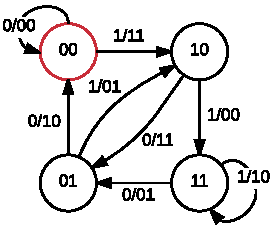
\includegraphics[width=0.25\textheight]{viterbi/states.pdf}
		\legend{Fonte: Autores.}
	\end{figure}
	O receptor, é claro, não tem conhecimento direto das transições do transmissor. Ele só pode ver a sequência de paridades recebidas, possivelmente corrompidas. Sua tarefa é determinar a \textbf{melhor} sequência possível de estados transmitidos que podem ter gerado a sequência de paridades. Essa tarefa é chamada de decodificação, que será detalhada a seguir.

	\paragraph*{Tabela Trellis}

	Como mencionado acima, o receptor deve determinar a \textbf{melhor} sequência de estados que o transmissor passou. Essa sequência forma um caminho dentro da máquina de estados, que pode ser deduzido pelo decodificador. Trellis é a estrutura derivada da máquina de estados, ela ajuda o decodificador a escolher os melhores caminhos para recuperar a mensagem. Um exemplo de tabela Trellis é dado na \autoref{figure:viterbi-trellis}.
	\begin{figure}[htb]
		\caption{\label{figure:viterbi-trellis}A tabela Trellis é útil para entender o processo de decodificação de uma máquina de estados.}
		\centering
		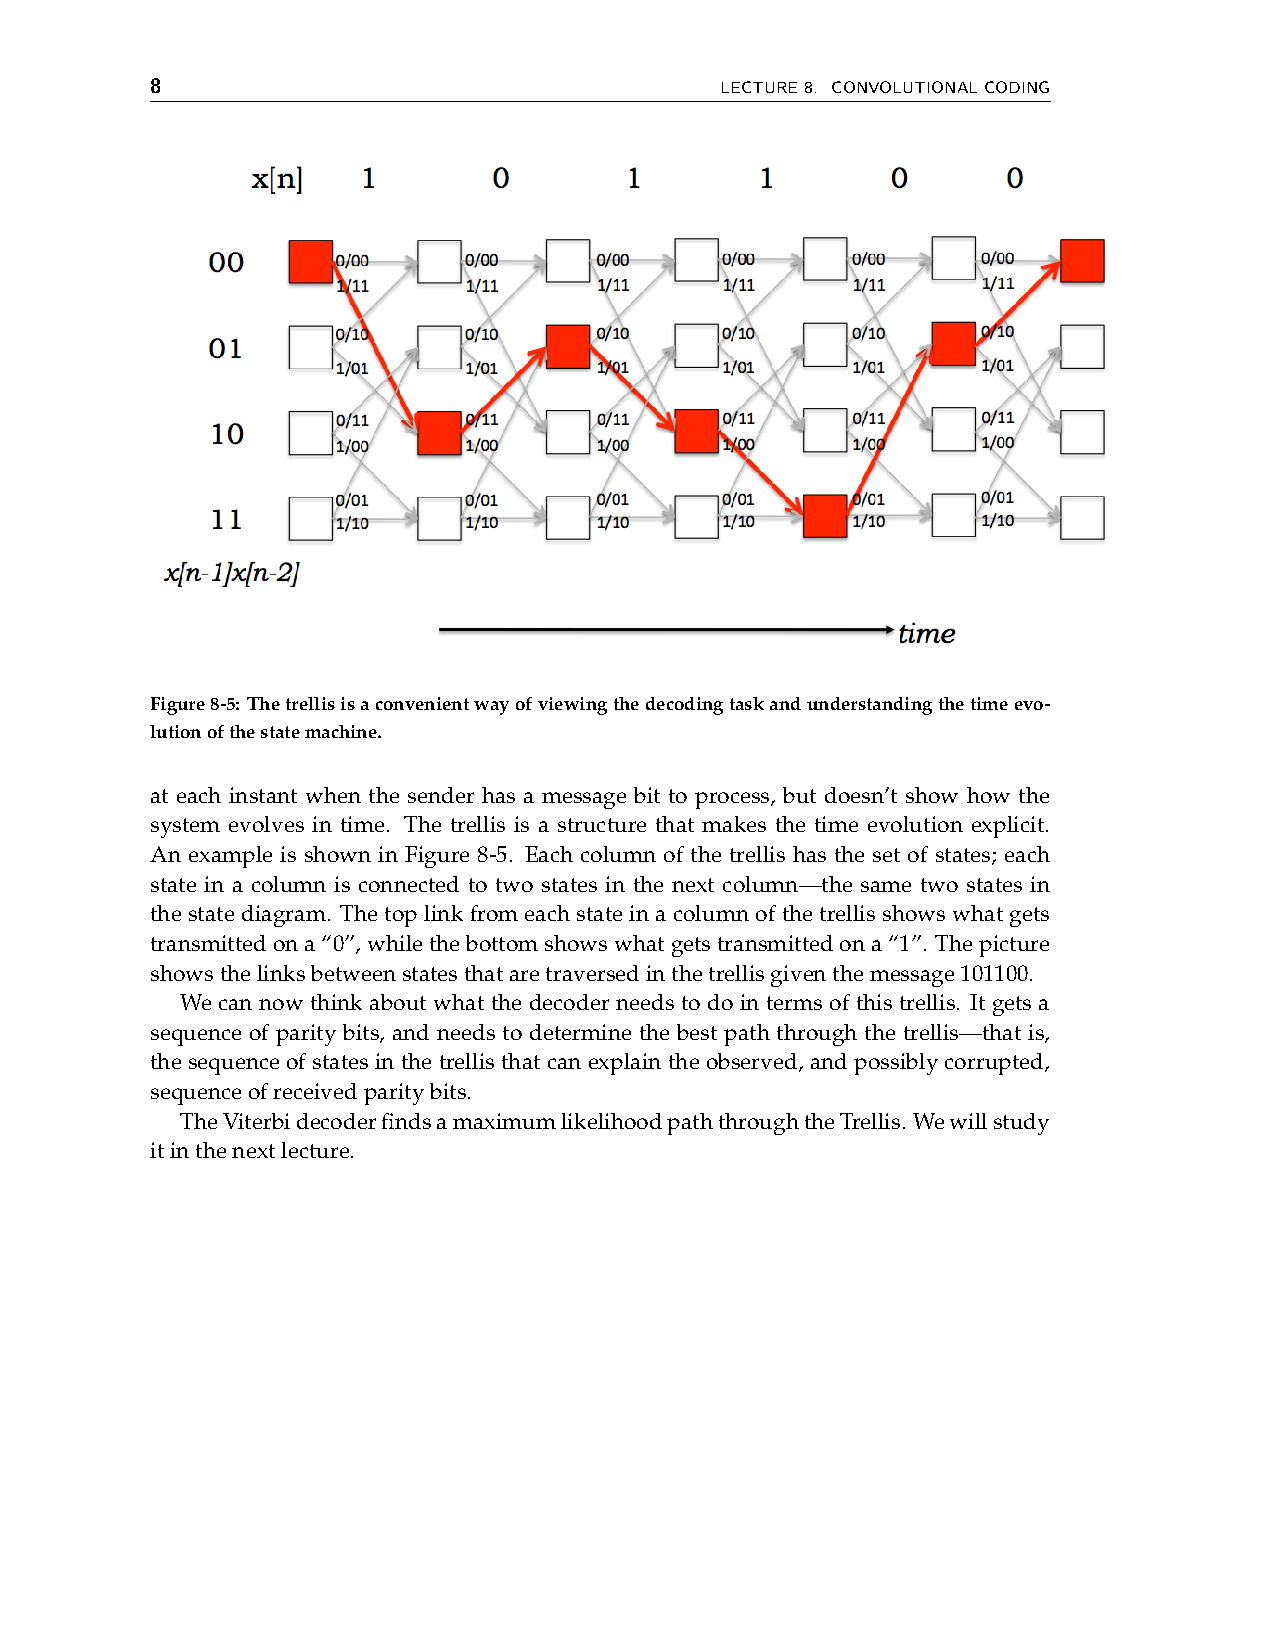
\includegraphics[width=0.6\textheight,trim={0cm 18cm 0cm 2.5cm},clip]{viterbi/trellis.pdf}
		\legend{Fonte: \cite{mit-convolutional}}
	\end{figure}
	Nessa figura, cada coluna tem um grupo de estados; cada estado é conectado a dois estados na próxima coluna; cada seta indica qual saída e próximo estado para cada entrada. A figura mostra o caminho percorrido pelo transmissor com a mensagem 101100.

	O decodificador deve identificar o melhor caminho utilizando a tabela Trellis, explicando por meio dela a sequência de paridades observadas e possivelmente corrompidas. Esse decodificador é chamado de Viterbi.

	\paragraph*{Algoritmo}
	O algoritmo de decodificação Viterbi é composto por três componentes principais: a métrica de ramificação (BM), a métrica de caminho (PM) e o \textit{Traceback Unit}.

	A métrica de ramificação calcula as distâncias entre a entrada e todas as possíveis entradas. Em alguns casos ela também é conhecida como distância de Hamming.

	A métrica de caminho calcula todos caminhos possíveis na tabela Trellis. Esse módulo é composto por múltiplos submódulos chamados ACS (Add, Compare and Select), que representam um estado e realizam a decisão de qual será o próximo estado. Após realizar a decisão, o ACS grava o caminho até o próximo estado e a distância acumulada na memória do \textit{Traceback Unit}. Esse processo se repete à medida que cada \textit{bit} da mensagem entra no Viterbi e apenas acaba quando a mensagem termina.

	Ao fim da mensagem, o \textit{Traceback Unit} escolhe o caminho com a menor distância acumulada e o percorre de forma invertida.

	\paragraph*{\textit{Fangled} Viterbi}

	Pode-se observar que esse método necessita de muitos recursos e computação, pois grava e compara todos os caminhos possíveis durante sua execução. O algoritmo pode ser simplificado removendo o módulo de \textit{Traceback Unit} e utilizando apenas uma unidade modificada de ACS. Essa unidade escolhe a menor distância de acordo com o estado atual e percorre o caminho, removendo a necessidade de gravar as possibilidades em memória. Esse método é chamado de \textit{Fangled} Viterbi.

	\subsubsection*{\textit{Deinterleaver}}

	O processo de \textit{deinterleaving} é análogo ao processo de \textit{interleaving} e é o único que não necessita de atenção especial para um estudo de um novo algoritmo.

	\subsubsection*{Decodificação \textit{Reed Solomon}}

	Esta seção discorre sobre as quatros etapas principais do processo de decodificação de Reed Solomon abordados na execução do projeto. Alguns dos algoritmos são discutidos com mais detalhes em \cite{reed-solomon-berle}.

	\paragraph*{Cálculo das síndromes}

	As síndromes são calculadas através da mensagem recebida e dos símbolos de paridade. O objetivo desse cálculo é identificar, num primeiro momento, a presença de erros no bloco que foi recebido em relação ao que foi transmitido. Utilizaremos aqui a notação de $R(x)$ para o bloco recebido e $E(x)$ para os possíveis erros. Portanto:

	\begin{equation}
	R(x) = C(x) + E(x)
	\end{equation}

	Caso a mensagem recebida não tenha erros, teremos $E(x)$ formado por 15 símbolos de 0000 no caso de Reed Solomon (15, 7). Se pelo menos um símbolo de $E(x)$ possuir pelo menos um \textit{bit} diferente de 0, configura-se um erro, e o cálculo das síndromes deverá apontá-lo. Caso o número de símbolos com erro exceda $t$, ou 4 símbolos para um código (15, 7), o erro será identificado nas síndromes, porém não será possível corrigi-lo posteriormente.

	No caso de Reed Solomon, as síndromes podem se definir da seguinte maneira:

	\begin{equation}
	S_{i} = Q_{i}(x)(x + \alpha^{i}) + R(x)
	\end{equation}

	No caso específico em que $x$ é $\alpha^{i}$, temos que o primeiro termo da soma é nulo, já que $x + \alpha^{i} = 0000$. Portanto:

	\begin{equation}
	S_{i} = R(\alpha^{i})
	\end{equation}

	E haverá um total de $2t$ síndromes, uma para cada raiz do polinômio codificador $G(x)$. Considerando que existem $v$ símbolos com erros, com $v \leq t$, teremos:

	\begin{equation}
	E(x) = V_{1}x^{L_{1}} + ... + V_{v}x^{L_{v}}
	\end{equation}

	Com $V_{i}$ representando os valores do erro, e $L_{i}$ indicando a localização desses erros. Portanto, para cada síndrome $S_{i}$:

	\begin{equation}
	S_{i}(\alpha^{i}) = V_{1}X_{1}^{i} + V_{2}X_{2}^{i} + ... V_{v}X_{v}^{i}
	\end{equation}

	Os valores de $X_{i}$ são usualmente designados para representar os localizadores de erro. Observe que os índices numéricos não necessariamente indicam o coeficiente do polinômio.

	Uma possível representação para o cálculo da síndrome, em hardware, seria a \autoref{Syndrome_logic}. Observe que cada símbolo $C_{j}$ do código é uma das entradas para cada ciclo do cálculo. O parâmetro $\alpha^{i}$ é fixo e seu índice é o mesmo da síndrome de saída. Portanto, para um código Reed Solomon (15, 7), existem 15 símbolos de entrada e 8 síndromes - uma para cada raiz do polinômio codificador.

	\begin{figure}[!htb]
		\caption{\label{Syndrome_logic} Módulo genérico de cálculo de uma das síndromes}
		\centering
		\includegraphics[width=0.2\textheight]{Syndrome.png}
		\legend{Fonte: Autores.}
	\end{figure}

	\paragraph*{Localização dos erros}

	O polinômio localizador de erros é construído com auxílio dos localizadores de erro, denotados por $X_{1}$ a $X_{v}$.

	\begin{equation}
	\Lambda(x) = (1 + xX_{1})(1 + xX_{2})...(1 + xX_{v})
	\end{equation}

	\begin{equation}
	\Lambda(x) =  1 + \Lambda_{1}x^{1} + ... + \Lambda_{v-1}x^{v-1} + \Lambda_{v}x^{v}
	\end{equation}

	Dessa forma teremos os inversos de $X_{1}$ a $X_{v}$ como raízes deste polinômio, sendo que cada uma dessas raízes torna $\Lambda(x)$ igual a zero.

	\begin{equation}
	\Lambda(X_{j}^{-1}) = \Lambda_{v}X_{j}^{-v} + ... + \Lambda_{1}X_{j}^{-1} + 1 = 0
	\end{equation}

	Multiplicando essa igualdade por $V_{j}*X_{j}^{i+v}$, temos:

	\begin{equation}
	Y_{j}X_{j}^{i+v} + \Lambda_{1}Y_{j}X_{j}^{i+v-1} + ... + \Lambda_{v}Y_{j}X_{j}^{i}
	\end{equation}

	Para diferentes valores de $j$, temos:
	\begin{equation}
	S_{i+v} + \Lambda_{1}S_{i+v-1} + ... + \Lambda_{v}S_{i} = 0
	\end{equation}

	Dessa forma, pode-se construir a seguinte matriz com um sistema de equações:

	\begin{equation}
	\begin{spmatrix}{}
	S_{v-1} & S_{v-2} & ... & S_{0} \\
	S_{v-1} & S_{v-2} & ... & S_{0} \\
	 ... & ... & & ...\\
	S_{2v-2} & S_{2v-3} & ... & S_{v -1} \\
	\end{spmatrix}
	\begin{spmatrix}{}
	\Lambda_{1} \\
	\Lambda_{2} \\
	...	 \\
	\Lambda_{v} \\
	\end{spmatrix}
	=
	\begin{spmatrix}{}
	S_{v}  \\
	S_{v+1}  \\
	...  \\
	S_{2v-1}  \\
	\end{spmatrix}
	\end{equation}

	\paragraph*{Algoritmo de Berlekamp-Massey}

	Resolvendo o sistema anterior, encontram-se os coeficientes do polinômio localizador de erros. Essa resolução pode se feita de várias formas, porém neste estudo foi selecionado o método de Berlekamp-Massey. Este algoritmo resolve o sistema por meio de aproximações sucessivas do polinômio localizador, iniciando com um $\Lambda(x)$ capaz de produzir $S_{v}$, ou a primeira síndrome. Conforme a seção anterior, calcula-se o próximo termo, $S_{v + 1}$, considerando:

	\begin{equation}
	S_{v + 1} = S_{v}\Lambda_{1} + S_{v-1}\Lambda_{2} + ... + S_{1}\Lambda_{v}
	\end{equation}

	Os valores de $\Lambda$ fazem parte da primeira aproximação. Caso esse valor da síndrome calculada pelo polinômio seja o mesmo valor da síndrome real, ou a diferença $d = 0000$, calcula-se $S_{v + 2}$. Caso contrário, o polinômio deve ser refinado:

	\begin{equation}
	\Lambda'(x) = \Lambda(x) +  Kx^{z}\Lambda''(x)
	\end{equation}

	$\Lambda''(x)$ é o último polinômio localizador estimado antes de haver uma diferença $d \neq 0000$. K é definida como $d''^{-1}d$, com $d''^{-1}$ sendo o inverso da diferença de quando o polinômio $\Lambda(x)$ foi modificado da última vez. Já $z$ é o número de estágios entre $\Lambda''^{+1}(x)$ e $\Lambda(x)$.

	Uma vez calculados os coeficientes do polinômio localizador,
	deve-se descobrir o valor de suas raízes. Como apontado anteriormente, o inverso destas aponta a localização dos erros. Esses valores são encontrados através do método de busca de Chien, que utiliza tentativa e erro, com todos os possíveis valores das raízes.

	\paragraph*{Valores dos erros}

	Existem diversas maneiras de encontrar os valores dos erros. O método abordado aqui - o algoritmo de Forney - utiliza o polinômio avaliador de erros, definido como:

	\begin{equation}
	\Omega(x) = \Omega_{v-1}x^{v-1} + ... + \Omega_{1}x + \Omega_{0}
	\end{equation}

	Os valores dos erros são dados por sua vez por:

	\begin{equation}
	V_{j} = X_{j}^{1-b} \frac{\Omega(X_{j}^{-1})}{\Lambda'(X_{j}^{-1})}
	\end{equation}

	$\Lambda'(x)$ é a derivada de $\Lambda(x)$, e $b$ é o índice do primeiro $\alpha$ usado no polinômio codificador, que neste caso será 0.

	\paragraph*{Síntese}

	Um decodificador de Reed Solomon pode ser dividido funcionalmente nos seguintes módulos:

	\begin{figure}[!htb]
		\caption{\label{RSDecoder_diagrama_logico} Diagrama funcional de decodificação Reed Solomon.}
		\centering
		\includegraphics[width=0.6\textheight]{RSdecoder_diagrama.png}
		\legend{Fonte: Autores.}
	\end{figure}

	Em suma, a entrada compreende os símbolos de mensagem e de paridade, que são enviados sequencialmente para o cálculo das síndromes. Uma vez calculadas as síndromes, seus valores são usados para se obter os polinômios localizador e avaliador de erros, cujos coeficientes determinam quando se realiza uma correção e qual o valor da correção que, somado à mensagem recebida, corrige-a.

	\paragraph*{Estratégia}

	O primeiro passo para aproximar os algoritmos de uma solução em hardware foi procurar níveis de abstração intermediários. O nível encontrado foi a programação em alto nível, reduzindo módulos como multiplicadores e somadores a funções. Uma das vantagens deste método foi a geração de saídas esperadas para cada módulo funcional, incluindo o bloco de saída final, corrigido ou a ser descartado. Esses dados foram fundamentais para a depuração e correções em hardware. Entretanto, uma das limitações deste método era a de que a linguagem de programação pertence a um paradigma diferente do da descrição de hardware, o que envolveu o uso de máquinas de estado no lugar de loops, por exemplo.

	\subsection{Estrutura da mensagem}

	Como neste trabalho apenas será implementado a camada física PHY I, a estrutura da mensagem não conterá elementos da camada MAC. Define-se portanto o elemento básico de transmissão, a Unidade de dados da camada física, ou PPDU, de acordo com a norma. Seu formato pode ser visto na \autoref{fig_ppdu_frame}.

	\begin{figure}[h]
		\caption{\label{fig_ppdu_frame} Estrutura da mensagem, composta pelo Cabeçalho de Sincronização (SHR), Cabeçalho da Camada Física (PHR) e Unidade de Dados de Serviço PHY (PSDU).}
		\centering
		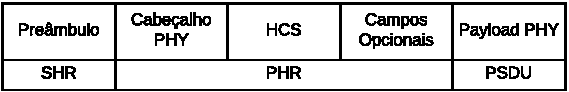
\includegraphics[width=0.5\textheight]{frame/PPDU.pdf}
		\legend{Fonte: Autores.}
	\end{figure}

	\subsubsection*{Preâmbulo - SHR}

	O campo de preâmbulo é usado pelo transmissor de data para obter sincronização ótica de \textit{clock} com uma mensagem recebida. A norma define um padrão de travamento rápido (FLP), seguido de quatro padrões dependentes da topologia (TDP) para fins de distinção de topologias de PHY diferentes. O preâmbulo deve ser enviado em uma taxa de \textit{clock} escolhida pelo transmissor e suportada pelo receptor. Ele é uma sequência de domínio de tempo e não possui nenhuma codificação de canal ou linha.

	O preâmbulo começa com um FLP com pelo menos 64 zeros e uns alternados. O FLP é fixado para iniciar com um padrão  \textbf{"1010..."} i.e., termina com um '0'. A sequência de transição máxima é usada para travar o circuito de recuperação de \textit{clock} e dados (CDR).

	O comprimento do padrão de travamento rápido não pode exceder o máximo de 16384 \textit{bits}. Após o FLP, quatro repetições de TDP devem ser enviados. O TDP deve conter 15 \textit{bits} de comprimento e deve ser invertido a cada repetição para providenciar \textit{DC balance}. O diagrama da estrutura do SHR está na \autoref{figure:SHR-frame}.

	\begin{figure}[h]
		\caption{\label{figure:SHR-frame}Estrutura do SHR - Cabeçalho da Camada Física.}
		\centering
		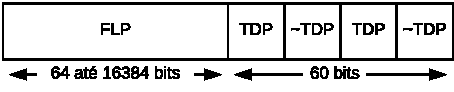
\includegraphics[width=0.4\textheight]{frame/SHR.pdf}
		\legend{Fonte: Autores.}
	\end{figure}

	O preâmbulo deve ser enviado utilizando modulação OOK (\textit{on-off keying}). O campo deve ser formatado com um TDP fixo e a lista de topologias está definida na \autoref{table:tdpdef}.

	\begin{table}[h]
		\caption{Definição de Topologias para o TDP.}
		\centering
		\begin{tabular}{c c c}
			\hline
			TDP & Topologia & Valor\\ \hline
			P1 & Independente & 1 1 1 1 0 1 0 1 1 0 0 1 0 0 0 \\
			P2 & Peer-to-peer & 0 0 1 0 1 1 1 0 1 1 1 1 1 1 0 \\
			P3 & Estrela & 1 0 0 1 1 0 0 0 0 0 1 0 0 1 1 \\
			P4 & Broadcast & 0 1 0 0 0 0 1 1 0 1 0 0 1 0 1 \\
			\hline
		\end{tabular}
		\label{table:tdpdef}
		\legend{Fonte: Figura 120 da norma 802.15.7}
	\end{table}

	\paragraph*{Sincronização de \textit{Clocks}}

	Se refere ao ato de sincronizar os \textit{clocks} de sistemas independentes. Para a transmissão de dados via luz, como ambos os módulos (receptor e transmissor) não estão conectados via cabo, o sinal de \textit{clock} não é compartilhado. Dessa forma, é certo dizer que eles estão fora de fase. Para isso a norma especifica o FLP, um sinal com período fixo utilizado pelo receptor para sincronizar seu \textit{clock} com o do transmissor.

	\subsubsection*{Cabeçalho PHY - PHR}

	\begin{table}[ht]
		\caption{Definição dos campos do cabeçalho PHY.}
		\centering
		\begin{tabular}{c c}
			\hline
			Campo do cabeçalho & Comprimento em Bits \\ \hline
			Modo de Burst & 1\\
			Número do Canal & 3\\
			MCS ID & 6\\
			Comprimento PSDU & 16\\
			Extensão de dimerização OOK & 1\\
			Campos Reservados & 5\\
			\hline
		\end{tabular}
		\label{table:phy-header-def}
		\legend{Fonte: Tabela 81 da norma 802.15.7}
	\end{table}

	O cabeçalho PHY, como mostrado na \autoref{table:phy-header-def}, deve ser transmitido utilizando modulação OOK. Ele deve ser enviado na menor velocidade listada da camada, que no caso de PHY I é 11.67kb/s e fica no cabeçalho como 000000.

	A maioria dos campos não será usada por motivos de redução de escopo, portanto o receptor e transmissor não terão habilitado o modo \textit{Burst}, canais e dimerização OOK. O único campo variável do cabeçalho será o Comprimento PSDU, que dependerá do conteúdo da mensagem enviada.

	\subsubsection*{Unidade de Dados de Serviço PHY - PSDU}

	Como o escopo do trabalho não engloba a camada MAC, o campo de PSDU conterá apenas a mensagem. A estrutura adaptada sem os cabeçalhos MAC está na \autoref{figure:PSDU-frame}. A norma ainda especifica \textit{tail bits} para reiniciar o processo do código convolucional.

	\begin{figure}[h]
		\caption{\label{figure:PSDU-frame}Estrutura do PSDU - Mensagem e \textit{tail bits}.}
		\centering
		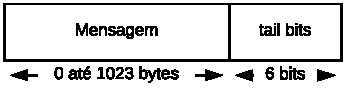
\includegraphics[width=0.4\textheight]{frame/PSDU.pdf}
		\legend{Fonte: Autores.}
	\end{figure}

	% ---
	\section{Hardware}\label{sec:method-hardware}
	% ---

	A seguir serão detalhadas as implicações da implementação da norma IEEE 802.15.7 em um escopo de hardware analógico, a partir da necessidade de transmitir, receber e converter sinais digitais em analógicos, que então serão convertidos de e para oscilações luminosas. A \autoref{figure:dataflow_analog_circuits} representa o fluxo dos dados:

	\begin{figure}[h!]
		\caption{\label{figure:dataflow_analog_circuits}Diagrama de blocos da conversão digital-analógica e analógica-digital da transmissão de dados.}
		\centering
		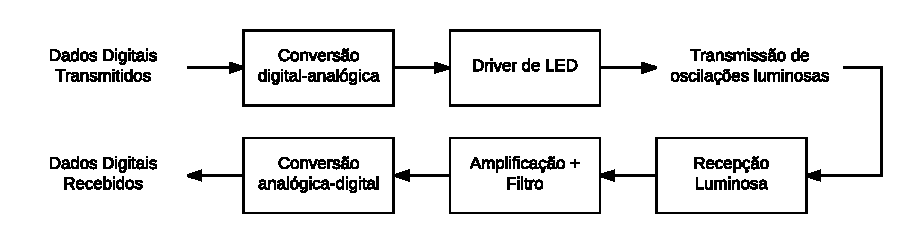
\includegraphics[width=0.6\textheight]{circuits/dataflow_analog_circuits.pdf}
		\legend{Fonte: Autores.}
	\end{figure}
	Os dois primeiros módulos são relativos ao circuito de recepção, enquanto os três últimos são relativos ao transmissor.

	% ---
	\subsection{Transmissão}
	% ---

	O transmissor do sistema de comunicação LiCy será composto por um conversor digital-analógico e um LED de potência. Os dados serão enviados a partir da FPGA e codificados em 0 e 3.3V, representando os sinais 0 e 1 digitais.

	Para cada um desses módulos deve haver um minucioso estudo sobre suas características eletro-eletrônicas, pois existem muitas restrições que devem ser levadas em conta com a frequência de operação $F_{op}$ = 200kHz, como:

	\begin{itemize}
		\item Amplificação de ruídos;
		\item Capacitâncias e Indutâncias parasitas em todos componentes, com ênfase no LED e no transistor;
		\item Prototipação dificultada, pois a \textit{breadboard} possui muita capacitância em seus contatos;
		\item Alta corrente para ligar um LED de potência.
		\item Componentes limitados pela frequência de operação.
	\end{itemize}

	Uma vez contornadas e solucionadas todas as restrições listadas acima, o circuito resultante deverá enviar sinais luminosos a uma frequência de 200kHz, que é a velocidade definida pela norma da camada PHY I.

	\subsubsection*{Conversor Digital-Analógico}\label{section:dac}
	Como o LED será de alta potência, a corrente necessária para ligá-lo corretamente é na ordem de grandeza de amperes. Essa corrente de polarização é incompatível com a fornecida pela porta de saída da FPGA (aproximadamente mil vezes menor). De forma a proteger o circuito da FPGA e também a chavear o LED, foi utilizado um transistor de potência.

	Além disso, deve-se notar que o método de modulação desejado é OOK (\textit{on-off keying}). Isso significa que, na presença de portadora (sinal 1), a luz deve estar ligada, enquanto em sua ausência (sinal 0), a luz deve estar desligada.

	\paragraph*{Curva característica de FET}

	Para projetar um circuito chaveador com um transistor de potência, é importante entender seu funcionamento. Um FET (\emph{Field Effect Transistor}) é um transistor que utiliza campo elétrico para controlar a condutividade de um tipo de carga de um canal em um semicondutor. Existem dois tipos de canais para transistores: n e p.

	Em um \textit{n-channel} FET, a aplicação de voltagem positiva no \textit{gate} em relação à \textit{source} permite a livre passagem de elétrons pelo caminho \textit{drain-source}. Analogamente, em um \textit{p-channel}, a aplicação de voltagem positiva no \textit{gate} bloqueia a passagem de elétrons. Nesse caso, a voltagem aplicada deve ser zero ou negativa para polarizá-lo. Esse comportamento deve ser melhor detalhado utilizando uma curva característica de transistores tipo FET.

	O gráfico \ref{figure:carac-mosfet} caracteriza a resposta $i_{D}$ do transistor tipo FET de acordo com a tensão $V_{GS}$ fornecida, indicando as regiões operação do componente. As regiões de interesse para o chaveamento do LED são as de saturação e corte, e serão detalhadas abaixo.

	\begin{chart}[h]
		\caption{\label{figure:carac-mosfet}Curva característica de um MOSFET, com indicações das regiões de saturação, corte e triodo.}
		\centering
		%  trim={<left> <lower> <right> <upper>}
		\includegraphics[page=8,width=0.4\textwidth, trim={16.5cm 9.89cm 3.6cm 3cm},clip]{circuits/Electronics_Ch5.pdf}
		\legend{Fonte: \cite{microelectronics-circuits}}
	\end{chart}

	\subparagraph*{Região de Corte}
	Na região de corte, o transistor se comporta como uma chave aberta. Esse comportamento é visto em todos transistores FET em que se aplica uma tensão $V_{GS} \leq V_{t}$, onde $V_{t}$ indica a tensão de limiar  característica de cada componente. A \autoref{figure:mosfet-cutoff} mostra um circuito com comportamento equivalente.

	\begin{figure}[h]
		\caption{\label{figure:mosfet-cutoff}Equivalência de circuitos com MOSFET em região de corte.}
		\centering
		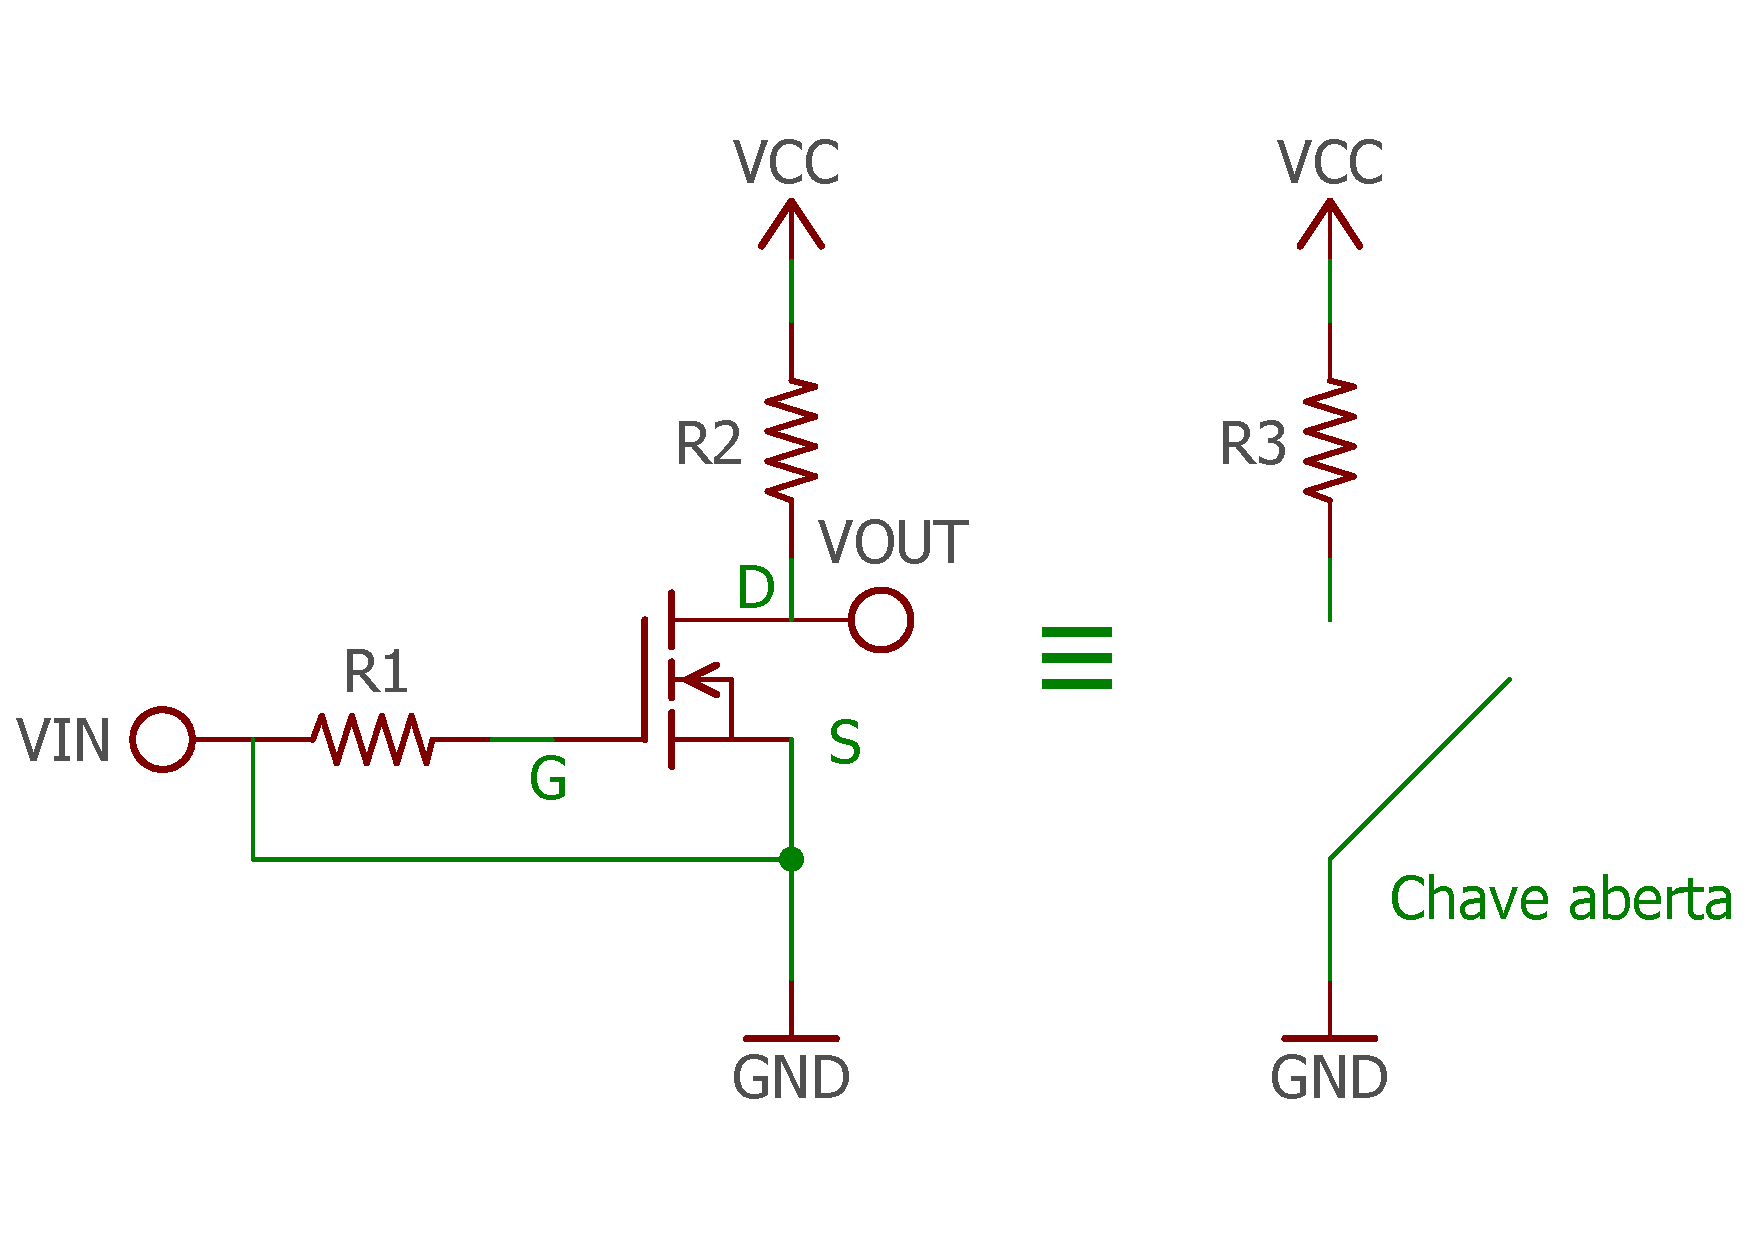
\includegraphics[width=0.5\textwidth, trim={0cm 2cm 0cm 2cm}, clip]{circuits/mosfet_cutoff.pdf}
		\legend{Fonte: Autores.}
	\end{figure}

	Nesse esquemático, R1 representa o resistor que controla a tensão no \textit{gate}, enquanto R2 e R3 representam a carga.

	Para a aplicação OOK, é interessante que a chave do LED esteja aberta quando a FPGA gerar um 0 digital. A restrição mínima da tensão de limiar é $V_{th} > 0V$, pois a FPGA não consegue gerar sinais negativos sem circuito auxiliar.

	\subparagraph*{Região de Saturação}

	Na região de saturação, o transistor se comporta como uma chave fechada. Em uma situação real, dependendo de qual $V_{GS} \geq V_{t}$ aplicado, é permitida maior ou menor passagem de corrente $i_{D}$, como pode-se observar na \autoref{figure:carac-mosfet}. Os valores $i_{D}$ não são fiéis à realidade, uma vez que um MOSFET de potência permite passagem de corrente muito maior. O esquemático na \autoref{figure:mosfet-saturation} mostra um circuito com FET na região de saturação com um circuito com comportamento equivalente, utilizando apenas componentes passivos.

	\begin{figure}[htb]
		\caption{\label{figure:mosfet-saturation}Equivalência de circuitos com MOSFET em região de saturação.}
		\centering
		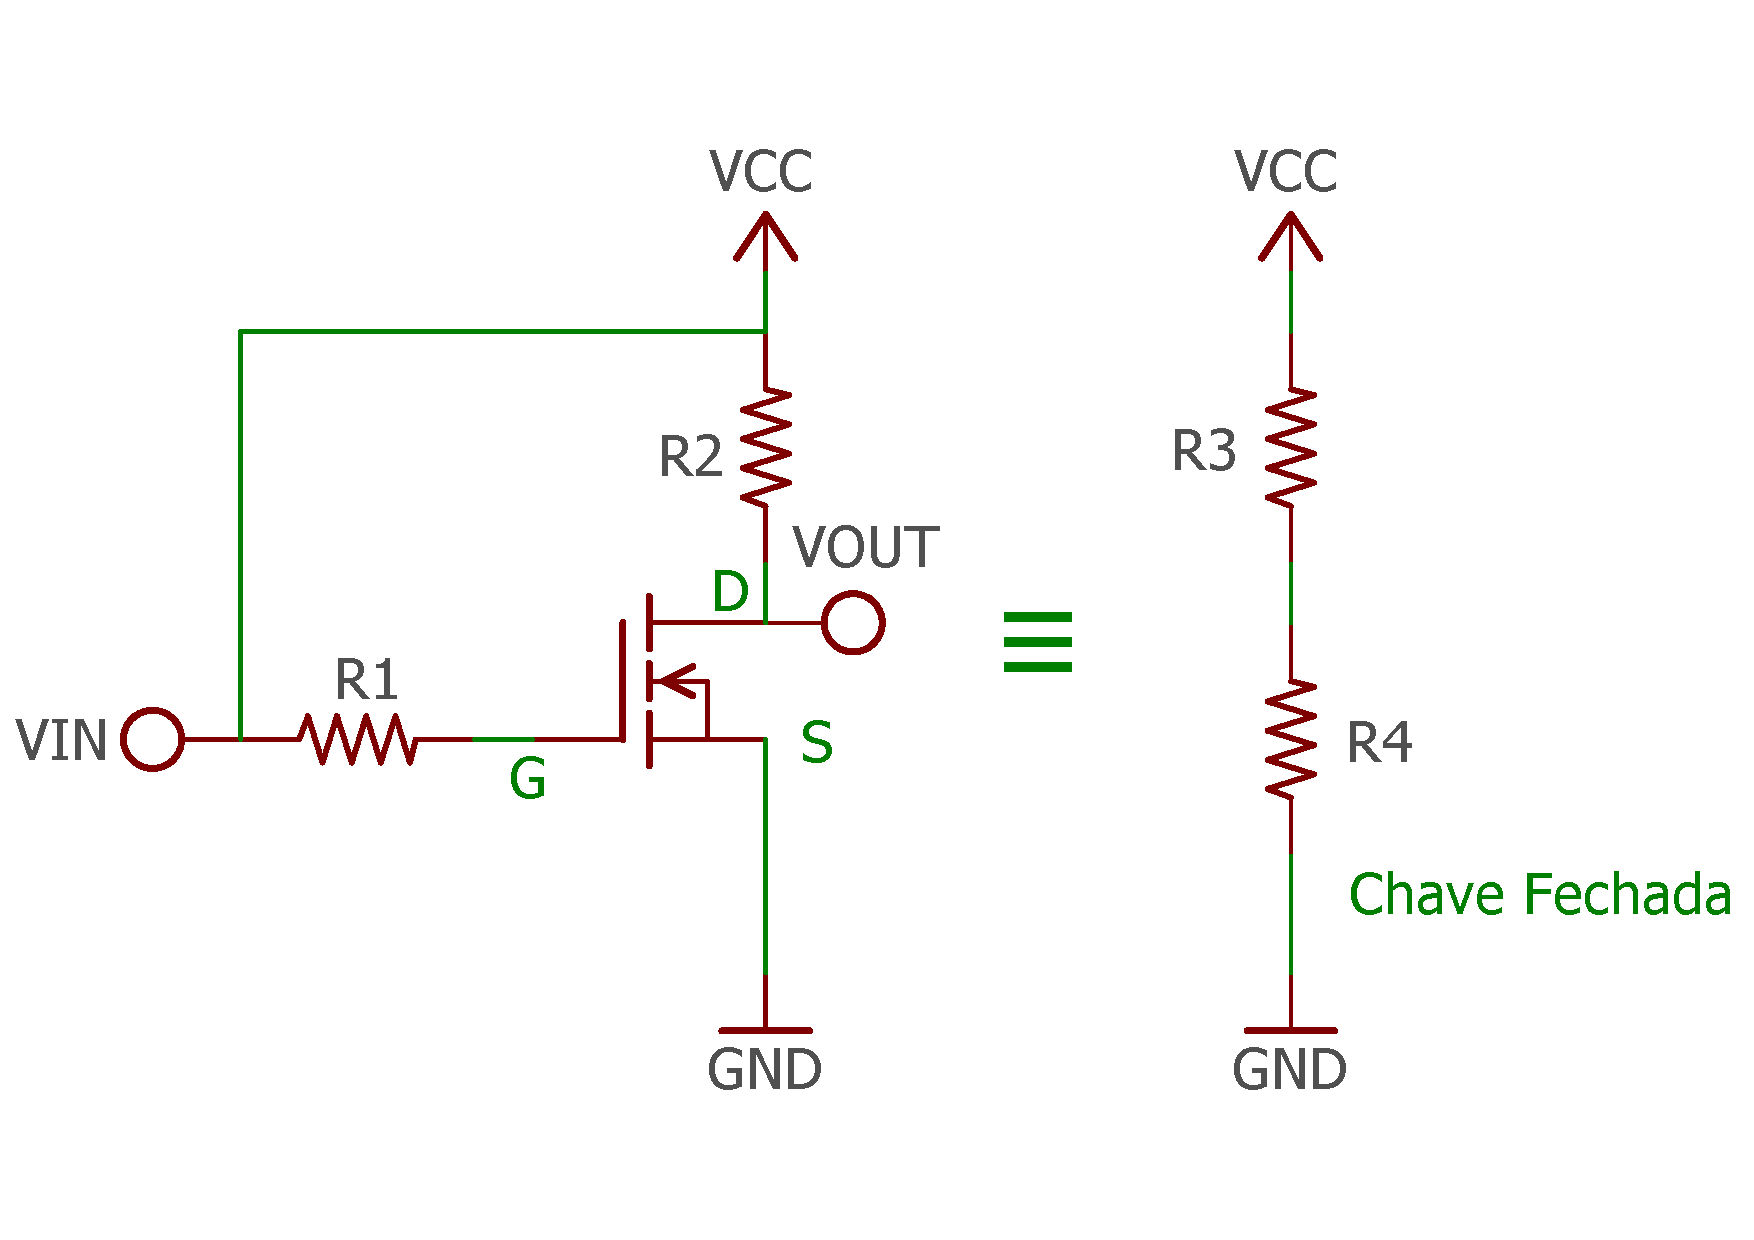
\includegraphics[width=0.5\textwidth, trim={0cm 2cm 0cm 2cm}, clip]{circuits/mosfet_saturation.pdf}
		\legend{Fonte: Autores.}
	\end{figure}

	Nesse esquemático, R1 representa o resistor que controla a tensão no \textit{gate}, enquanto R2 e R3 representam a carga e R4 a resistência interna $R_{DS}$ do MOSFET.

	\paragraph*{Conclusão}

	O transistor deve ser deixado na configuração de fonte comum da \autoref{figure:fet-common-source}, agindo como chave entre o circuito do LED, VCC e GND. Quando a FPGA gerar o sinal digital 1, o circuito deve atender $V_{in} \geq V_{(i_{D} > Corrente de LED aceso)}$. Da mesma forma, quando o sinal gerado for 0, é necessário projetar  $V_{in} < V_{i_{D} \approx 0}$.

	\begin{figure}[h]
		\caption{\label{figure:fet-common-source}FET-n em modo de fonte comum.}
		\centering
		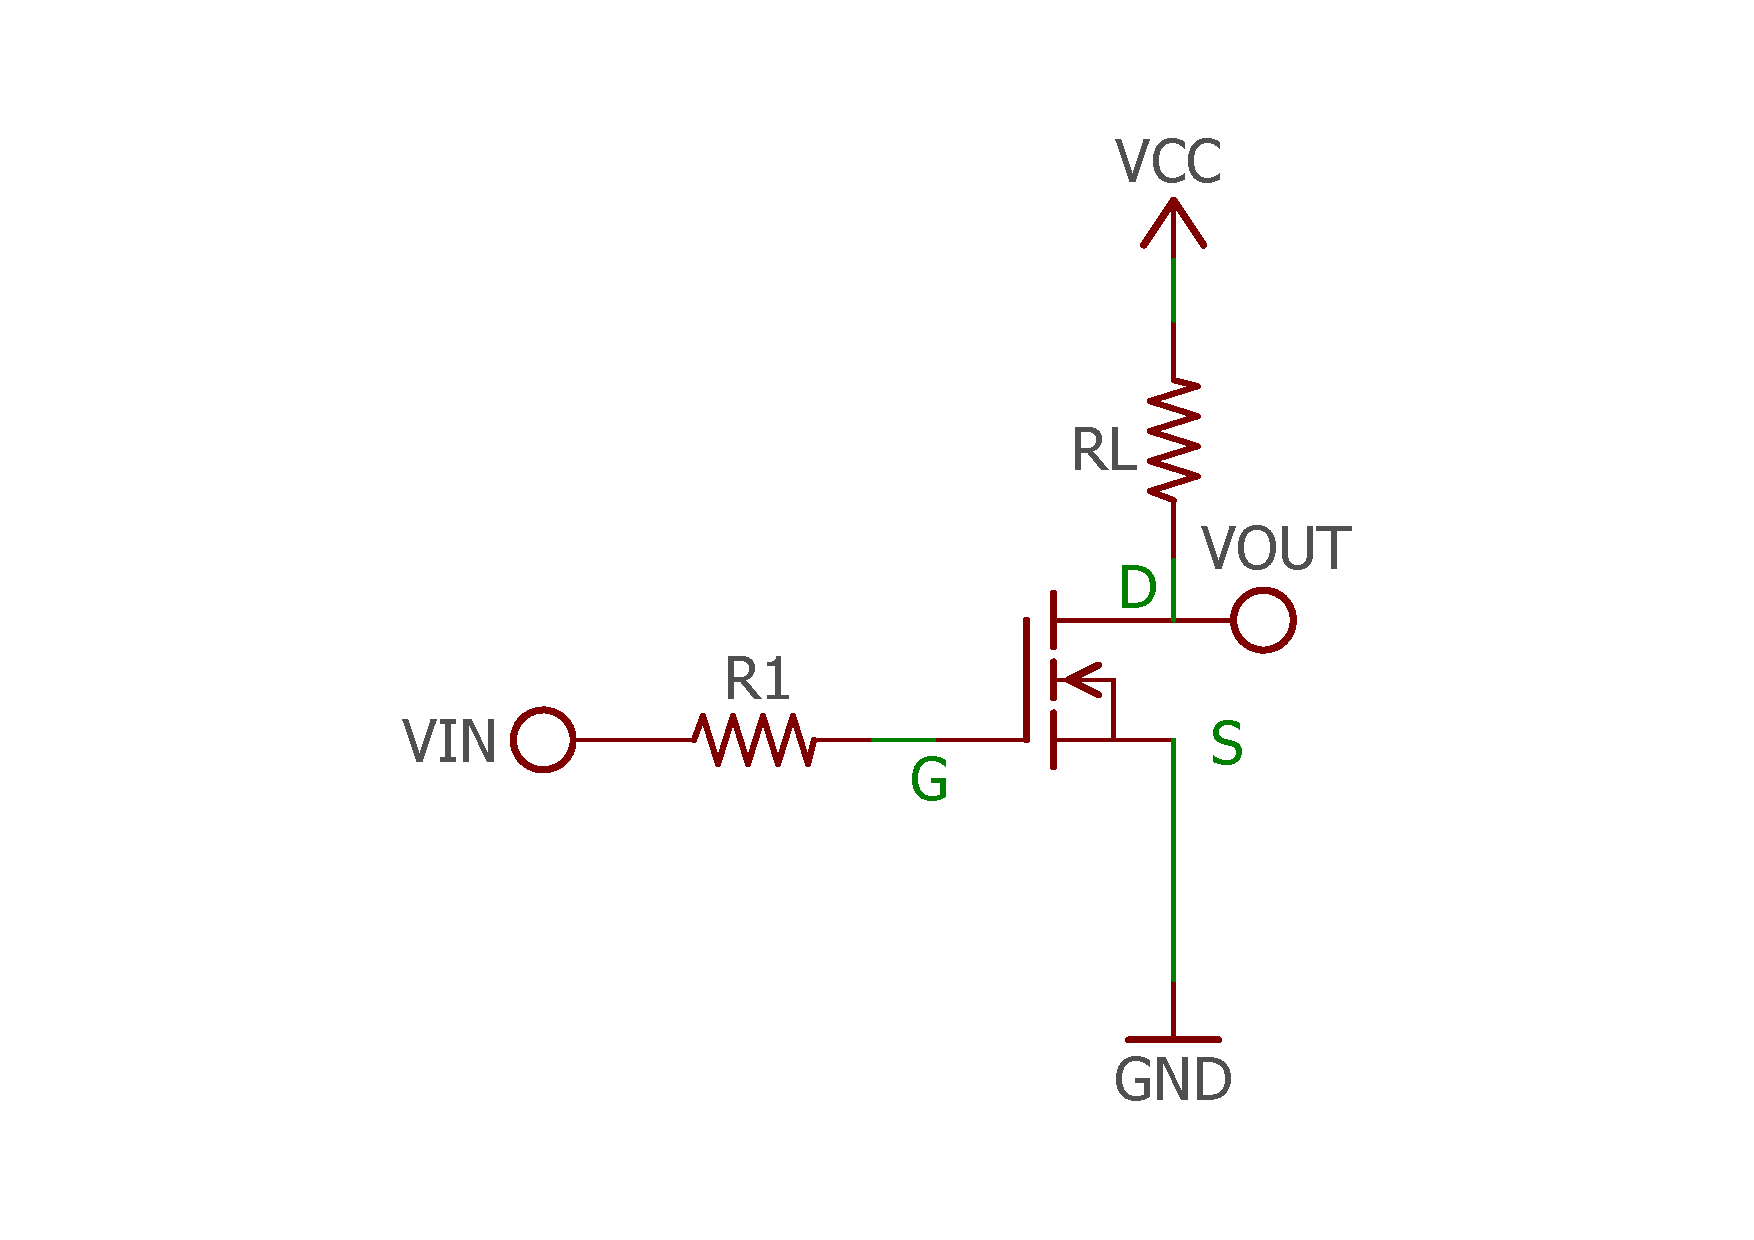
\includegraphics[width=0.5\textwidth, trim={0cm 2cm 0cm 2cm}, clip]{circuits/mosfet_example.pdf}
		\legend{Fonte: Autores.}
	\end{figure}

	% ---
	\subsubsection*{LED}\label{method-hardware-led}
	% ---

	De acordo com a \autoref{tab_phy1} é necessário suportar uma frequência de oscilação luminosa mínima de 200kHz. Para não tornar o LED limitante, seria interessante se ele também suportasse a frequência de transmissão de 120MHz, que é a frequência para PHY II. Além disso, ele deve realizar a transmissão de luz a distâncias de pelo menos um metro, conforme requisito funcional do projeto.

	Será então necessária a utilização de um LED de potência. É muito importante que o LED escolhido tenha resposta luminosa de acordo com o chaveamento, de forma que a tensão fornecida seja proporcional à luz emitida. Como o grupo não tem nenhum medidor de intensidade luminosa, será muito difícil de caracterizar um problema dessa natureza como, por exemplo, a possibilidade de o LED atrasar em relação a excitações em seus terminais. O circuito polarizador de um LED de alta potência pode ser simples, apenas ligando-o a um resistor de alta potência chamado de resistor limitador de corrente, como na \autoref{figure:led-circuit}.

	\begin{figure}[htb]
		\caption{\label{figure:led-circuit}Circuito polarizador de LED, com resistor limitador de corrente.}
		\centering
		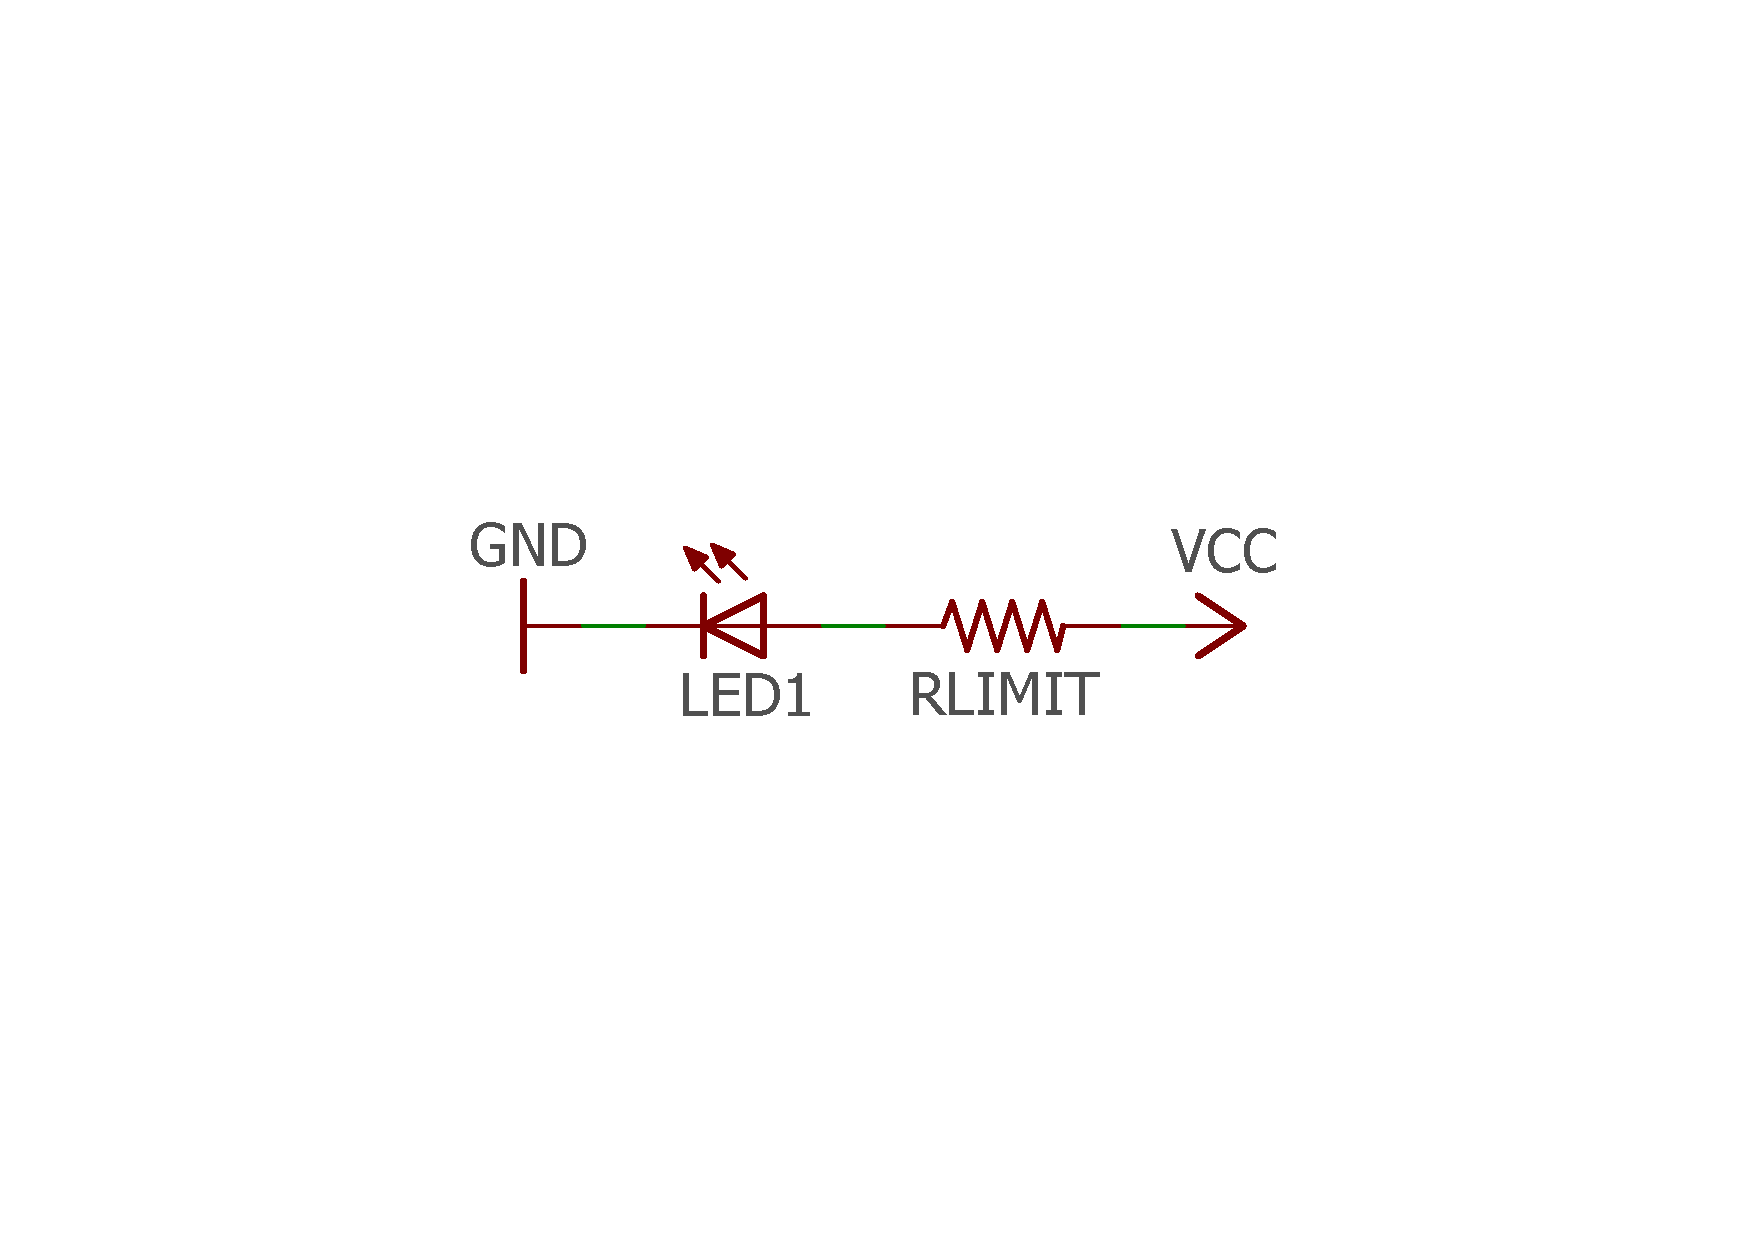
\includegraphics[width=0.5\textwidth, trim={8cm 8cm 8cm 8.5cm},clip]{circuits/led_circuit.pdf}
		\legend{Fonte: Autores}
	\end{figure}

	A corrente que passa pelo LED, que não pode exceder valores definidos de fábrica, pode ser calculada pela fórmula:
	\begin{equation}
	V_{LED} = \frac{V_{CC}}{R_{limit}}
	\end{equation}

	\paragraph*{Resposta Luminosa}

	Como definido no próprio nome, o LED é um Diodo Emissor de Luz. Então, para efeitos de simulação, pode-se considerar que ele é um diodo (\autoref{figure:led-schematic}).

	\begin{figure}[h]
		\caption{\label{figure:led-schematic}Símbolo esquemático de um LED, similar ao do diodo.}
		\centering
		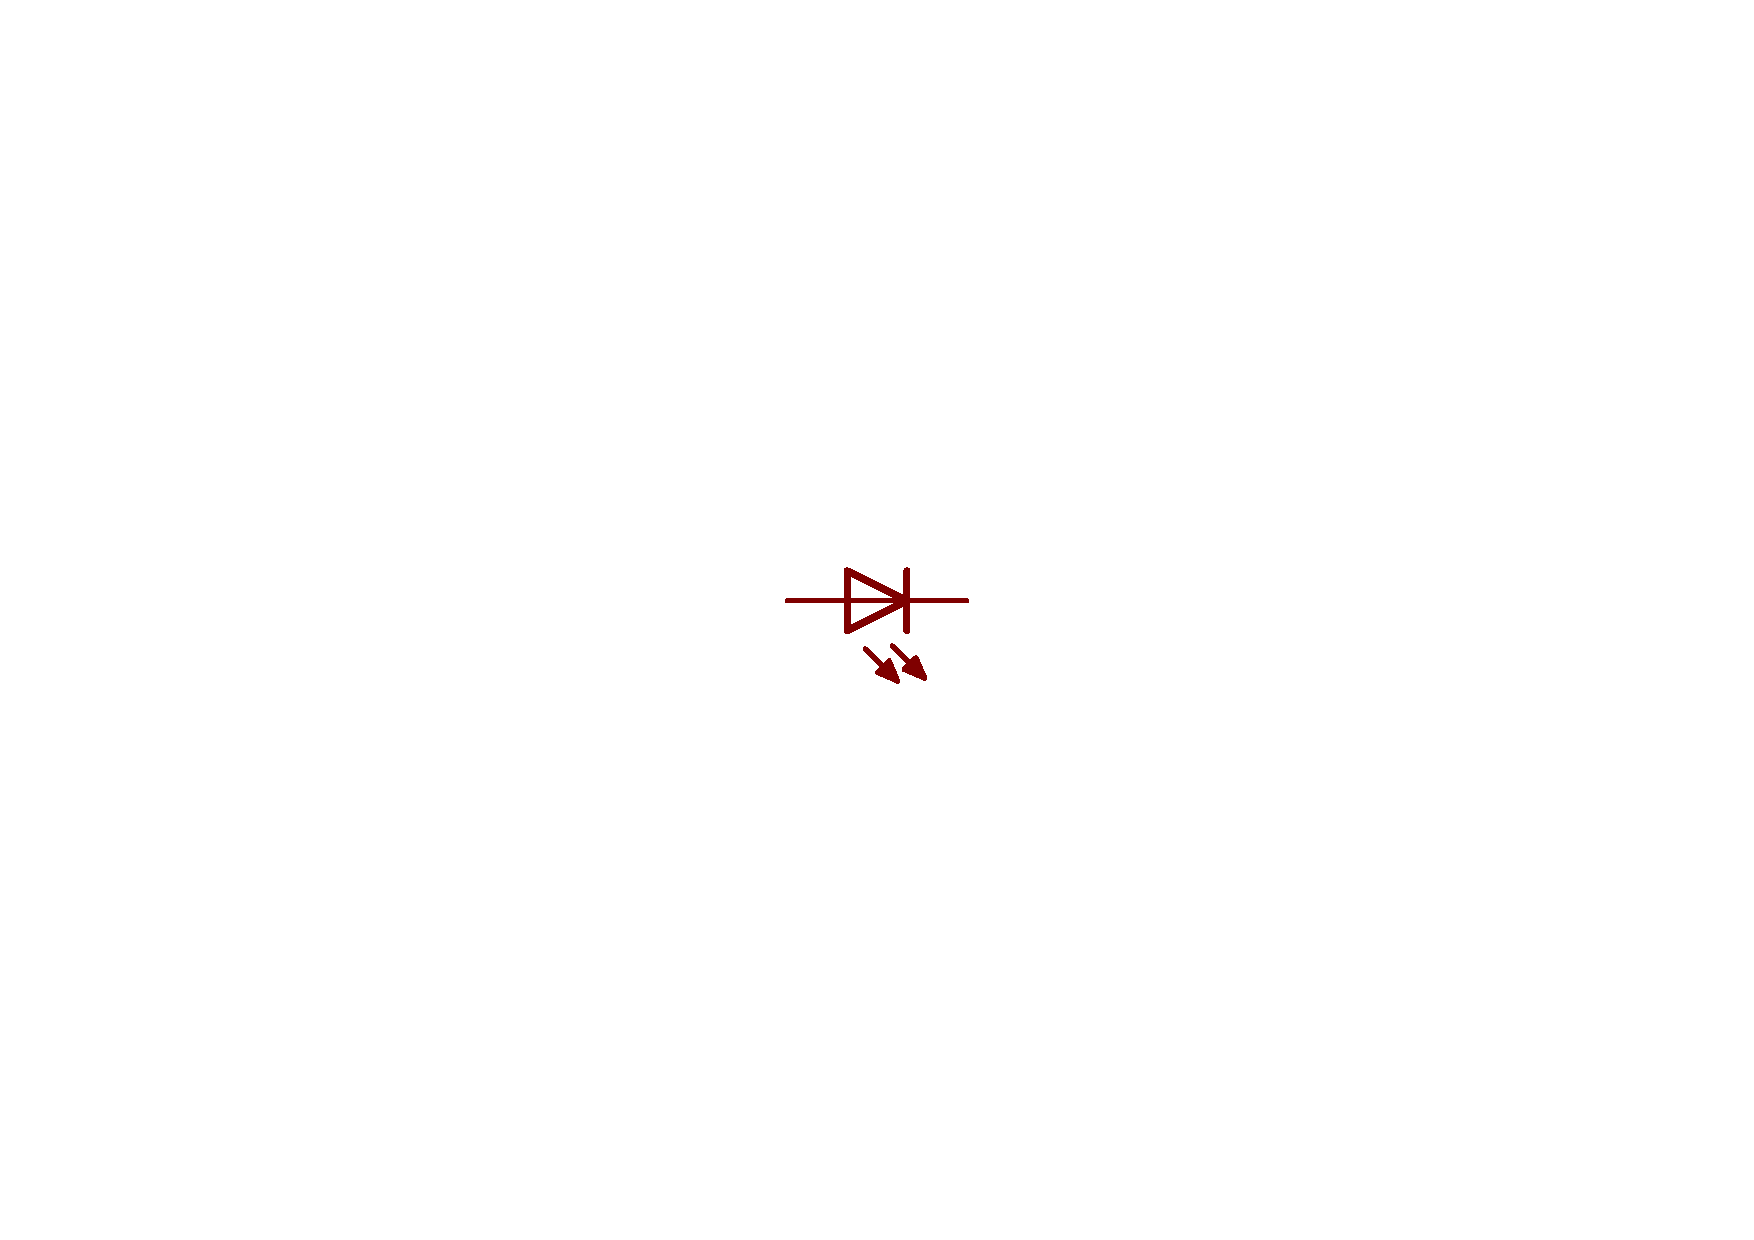
\includegraphics[width=0.3\textwidth, trim={12cm 9.2cm 12cm 9.5cm},clip]{circuits/led_schematics.pdf}
		\legend{Fonte: Autores.}
	\end{figure}

	O circuito proposto visa oscilar todos os componentes a 200kHz. Isso significa oscilar entre a região de saturação e corte. Ao realizar o fechamento ou abertura de seus terminais, é possível que o componente responda com efeitos de um capacitor. As componentes capacitivas passivas e ativas dos componentes criam respostas indesejadas no circuito. Para atenuá-las, é possível utilizar um filtro, que remove esse comportamento indesejado, aplicando uma onda de acordo com a entrada (da FPGA) no LED.

	Ainda existe outra opção para não gerar a componente capacitiva ativa no circuito: oscilar a voltagem de entrada apenas dentro da região de saturação do LED. Essa modificação consiste em aplicar uma componente contínua $V_{DC}$ no LED e uma alternada $V_{AC}$ pequena com a portadora do sinal gerado pela FPGA. Isso é muito utilizado em circuitos de fibra ótica, utilizando um componente chamado \textit{Bias-Tee}.

	\begin{chart}[htb]
		\caption{\label{figure:diode-carac}Zona de operação do diodo.}
		\centering
		\includegraphics[page=5,width=0.6\textwidth, trim={16cm 2.5cm 2cm 12.5cm}, clip]{circuits/Electronics_Ch3.pdf}
		\legend{Fonte: \cite{microelectronics-circuits}}
	\end{chart}

	No gráfico \ref{figure:diode-carac} é possível observar a curva de operação do diodo crescente. Ao submetê-lo a uma tensão, há resposta em $I_{D}$, que no caso do LED corresponde a intensidade luminosa. Cada diodo (ou LED) tem sua curva, e será necessário projetar o circuito levando esses parâmetros em consideração.

	No entanto, é possível que essa estratégia cause modificações também no circuito do receptor, pois o LED deixará de apagar e acender, apenas oscilando sua intensidade.

	% ---
	\subsection{Recepção}
	% ---

	É de responsabilidade do receptor realizar três processos: (i) a recepção dos sinais luminosos, (ii) sua amplificação com filtragem e (iii) a conversão das ondas em sinais digitais. Com o funcionamento pleno deles, será possível receber um sinal equivalente ao transmitido pela FPGA. Os processos e todos os métodos envolvidos serão explicados em detalhes a seguir nas seções \ref{section:light-reception}, \ref{section:adc},  \ref{section:highpass-filter}, \ref{section:dc-bias} e \ref{section:band-filter}.

	\subsubsection*{Recepção Luminosa}\label{section:light-reception}

	O módulo de recepção luminosa é o mais crítico do receptor, pois recebe oscilações luminosas e as converte em sinais analógicos. É muito empregado em circuitos receptores de fibra óptica, CD players, televisões, câmeras e até em medidores de batimento cardíaco. Os fotorreceptores mais comuns são fototransistores ou fotodiodos, que são classificados principalmente de acordo com sua velocidade de chaveamento.

	Um fototransistor é composto por um transistor de junção que responde à incidência de luz gerando e amplificando corrente elétrica. Seu tempo de resposta é da ordem de $\mu$s. Já o fotodiodo é um diodo semicondutor que gera diferença de potencial ou mudança em sua resistência quando iluminado, com o tempo de resposta usualmente em ns, devido a sua natureza semicondutora e arquitetura de silício.

	Para o projeto, é mais interessante a escolha do fotodiodo, pois possui alta velocidade de resposta, tornando a onda recebida o mais fiel possível à realidade.

	O fotodiodo tem dois principais modos de operação, com as seguintes características na \autoref{table:photodiode-comp}.

	\begin{table}[ht]
		\caption{Comparação entre modos de operação do fotodiodo.}
		\centering
		\begin{tabular}{c c c}
			\hline
			Modo de Operação  & Polarização & Características \\ \hline
			Fotovoltaico & não & $I_{dark}$ menor, resposta lenta \\
			Fotocondutivo & negativa & $I_{dark}$ maior, resposta rápida \\ \hline
		\end{tabular}
		\legend{Fonte: Autores.}
		\label{table:photodiode-comp}
	\end{table}

	Como velocidade de resposta é prioritária na aplicação de comunicação, será utilizado o modo fotocondutivo. A polarização reversa aumenta o comprimento da região de depleção e diminui a capacitância de junção, aumentando a performance em altas frequências.

	Mas como o fotodiodo apenas altera a corrente de polarização propocionalmente à luz que recebe, portanto é necessário convertê-la em tensão para amplificar o sinal e filtrar os eventuais ruídos. A conversão será feita por um amplificador de transimpedância.

	\paragraph*{Amplificador de Transimpedância}

	O comportamento de um amplificador de transimpedância é simples: converter corrente em tensão. Ele normalmente é utilizado com componentes em que a resposta em corrente é mais linear que a resposta em tensão, como no caso do fotodiodo.

	O amplificador apresenta baixa impedância de entrada para isolar o fotodiodo da voltagem de saída. Em relação à saída, ao contrário do fototransistor, que tem corrente de saída a $\mu$A, o fotodiodo gera uma corrente na ordem de grandeza de pA. Para converter essa corrente baixa em voltagem útil para o circuito, é necessário realizar a amplificação desse sinal utilizando um resistor de feedback $R_{F}$, rotulado como R1 na \autoref{figure:transimpedance-amp-simple}.

	\begin{figure}[h]
		\caption{\label{figure:transimpedance-amp-simple}Circuito Amplificador de Transimpedância.}
		\centering
		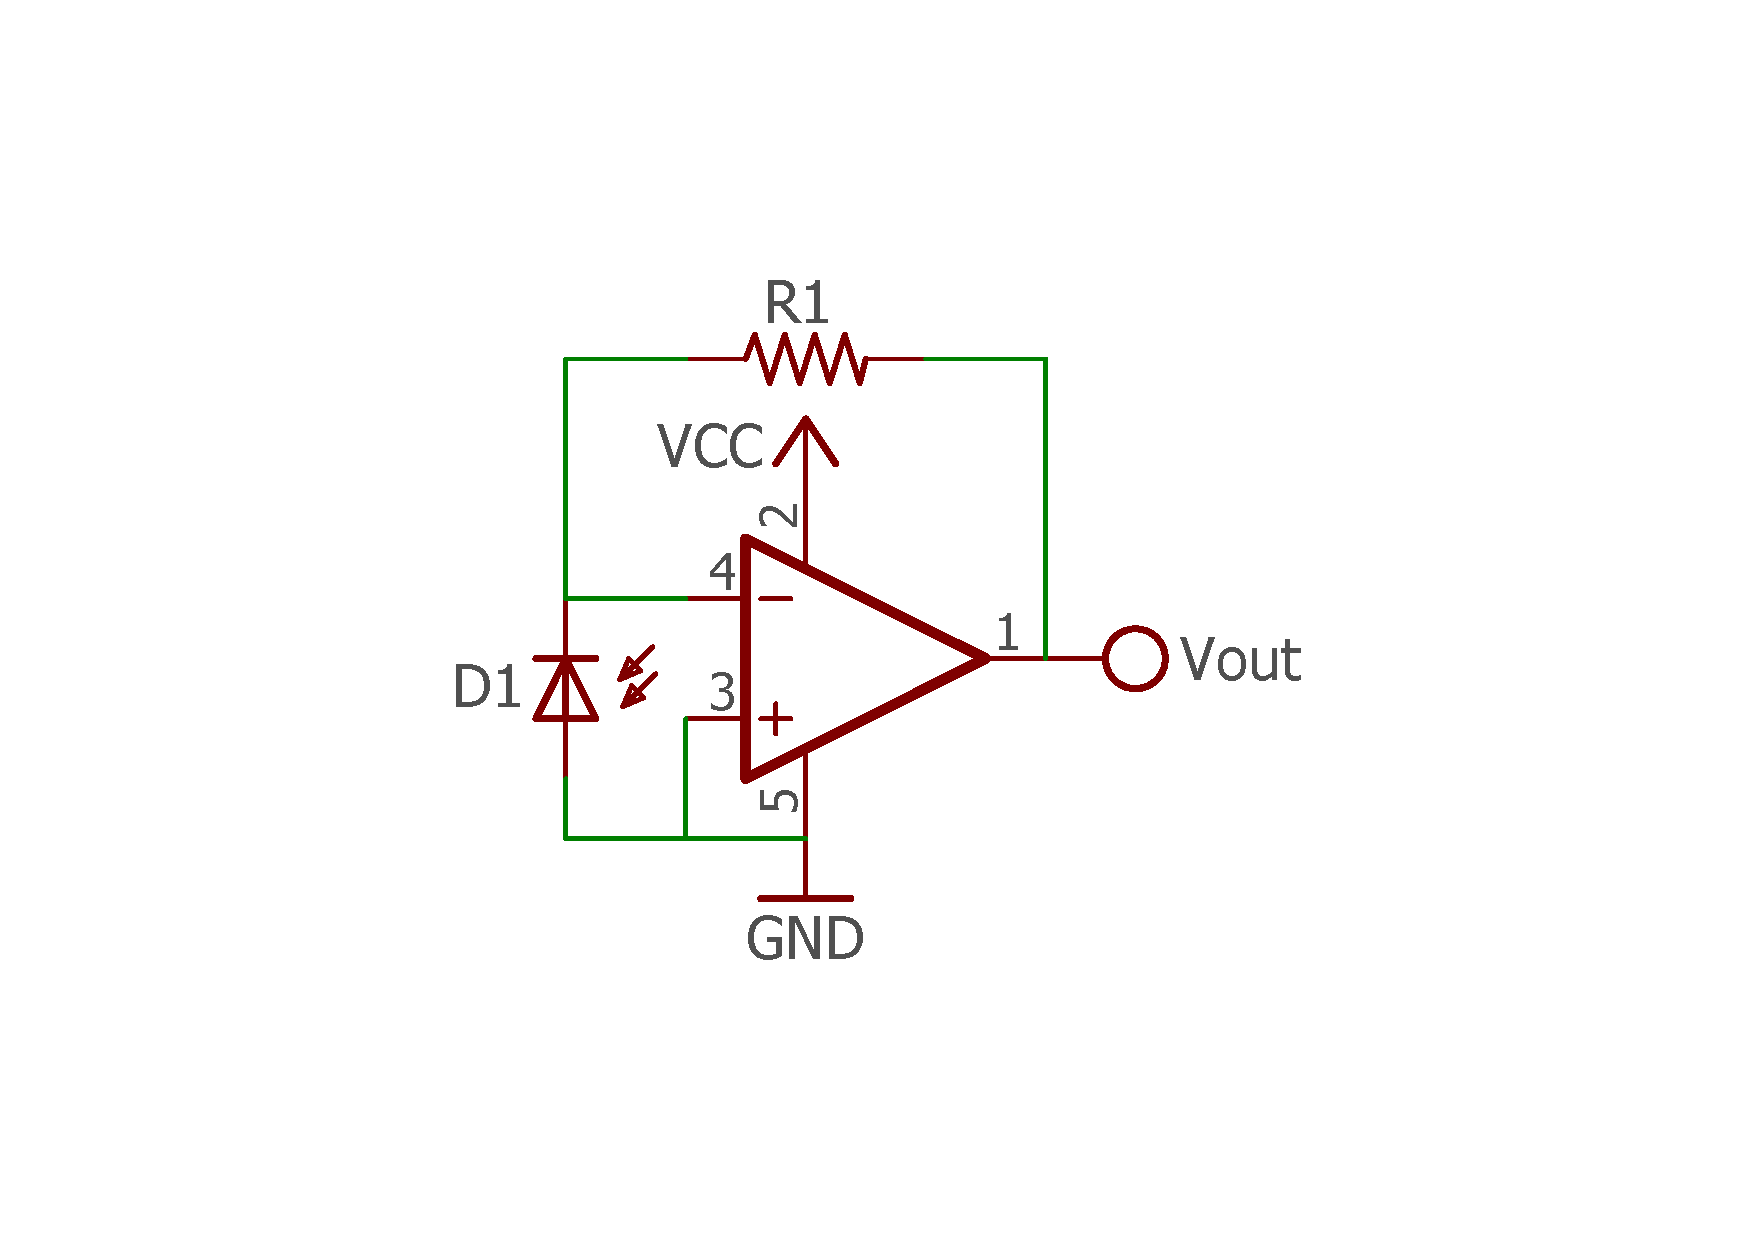
\includegraphics[width=0.6\textwidth, trim={2cm 3.8cm 2cm 3.8cm}, clip]{circuits/transimpedance_amp_simple.pdf}
		\legend{Fonte: Autores.}
	\end{figure}

	O ganho de amplificação é dado pela fórmula:

	\begin{equation}
	V_{out} = - I_{fotodiodo} \cdot R_{feedback}
	\end{equation}

	Como $I_{fotodiodo}$ é da ordem de pA, $R_{F}$ deve ser grande (M$\Omega$) para tornar a voltagem compatível com níveis TTL. Nota-se que $V_{out}$ é negativo pois o amplificador se encontra na configuração inversora. O gráfico \ref{plot:post-tia} ilustra o comportamento da saída do Amplificador de Transimpedância.

	\begin{chart}[h!]
		\caption{\label{plot:post-tia}Saída esperada do Amplificador de Transimpedância, com amplitude de $i_{D} \cdot R_{F}$, com componente $V_{DC} = L$ variável.}
		\centering
		\begin{tikzpicture}
		\begin{axis}[
		xmin=0, xmax=25,
		ymin=0, ymax=2,
		axis lines=middle,
		xticklabels={,,},
		ytick={0.3, 1, 1.7},
		yticklabels={$L-A_{i_{D} \cdot R_{F}}$,$L$,$L+A_{i_{D} \cdot R_{F}}$},
		%ylabel near ticks,
		%			ylabel style={yshift=-0.5cm},
		xlabel shift = 2 pt,
		xlabel style={yshift=-1cm},
		xlabel={[$t$]},
		ylabel={[$V_{out}$]}
		]
		\addplot[smooth, domain=0:8*pi, color=red]{0.7*sin(deg(x/2)) + 1};
		\addplot[domain=0:8*pi]{1};
		\end{axis}
		\end{tikzpicture}
		\legend{Fonte: Autores.}
	\end{chart}

	Após esse estágio de recepção, obtém-se uma onda com componente $V_{DC} = L$. Esse componente é variável e depende de alterações na intensidade de luz, variações na distância do transmissor com receptor, entre outros fatores. A amplitude da onda depende da corrente  $i_{D}$ do fotodiodo e da resistência de feedback $R_{F}$ do circuito amplificador.

	\subsubsection*{Conversor Analógico-Digital}\label{section:adc}

	Para poder realizar estágios adicionais de amplificação e comparação a fim de obter uma saída compatível com a entrada da FPGA, deve-se entender o funcionamento de um comparador. O circuito comparador utiliza um amplificador operacional com alto ganho sem realimentação e recebe dois sinais: uma voltagem de entrada $V_{in}$ e uma voltagem de referência $V_{ref}$. Ele realiza a comparação do nível de tensão analógico $V_{in}$ com $V_{ref}$ e produz saída de acordo com essa comparação. Seu desenho esquemático pode ser visto na \autoref{fig_comparator_circuit} e o comportamento de sua saída na \autoref{table:comparator-behaviour}.

	\begin{figure}[htb]
		\caption{\label{fig_double_comparator}Comparador e curva de resposta.}
		\begin{subfigure}{.5\textwidth}
			\caption{\label{fig_comparator_circuit}Circuito comparador simples.}
			\centering
			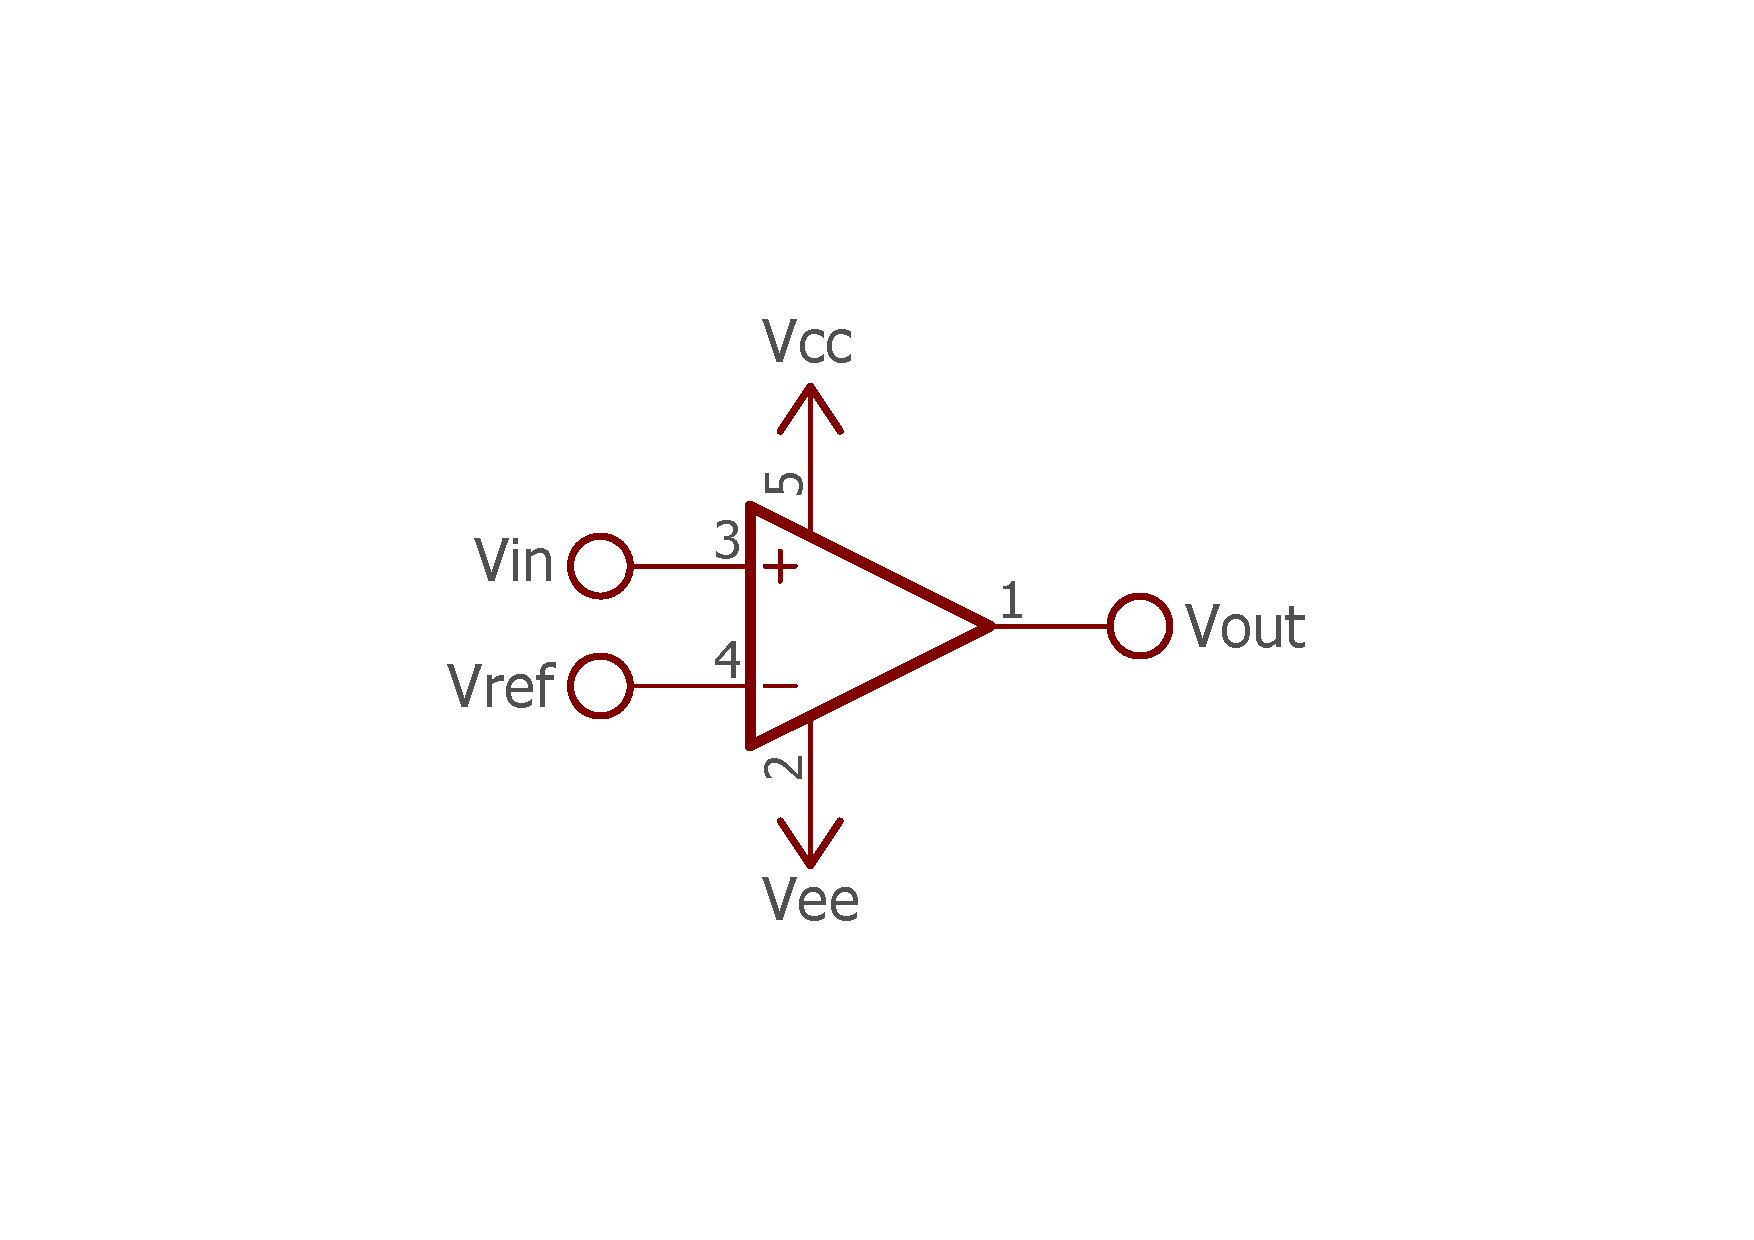
\includegraphics[width=0.77\textwidth, trim={7.5cm 5cm 7.5cm 5.5cm},clip]{circuits/comparator_amp.pdf}
			\legend{Fonte: Autores.}
		\end{subfigure}
		\begin{subfigure}{.5\textwidth}
			\caption{\label{fig_comparator_transfer}Curva de resposta de comparador real.}
			\centering
			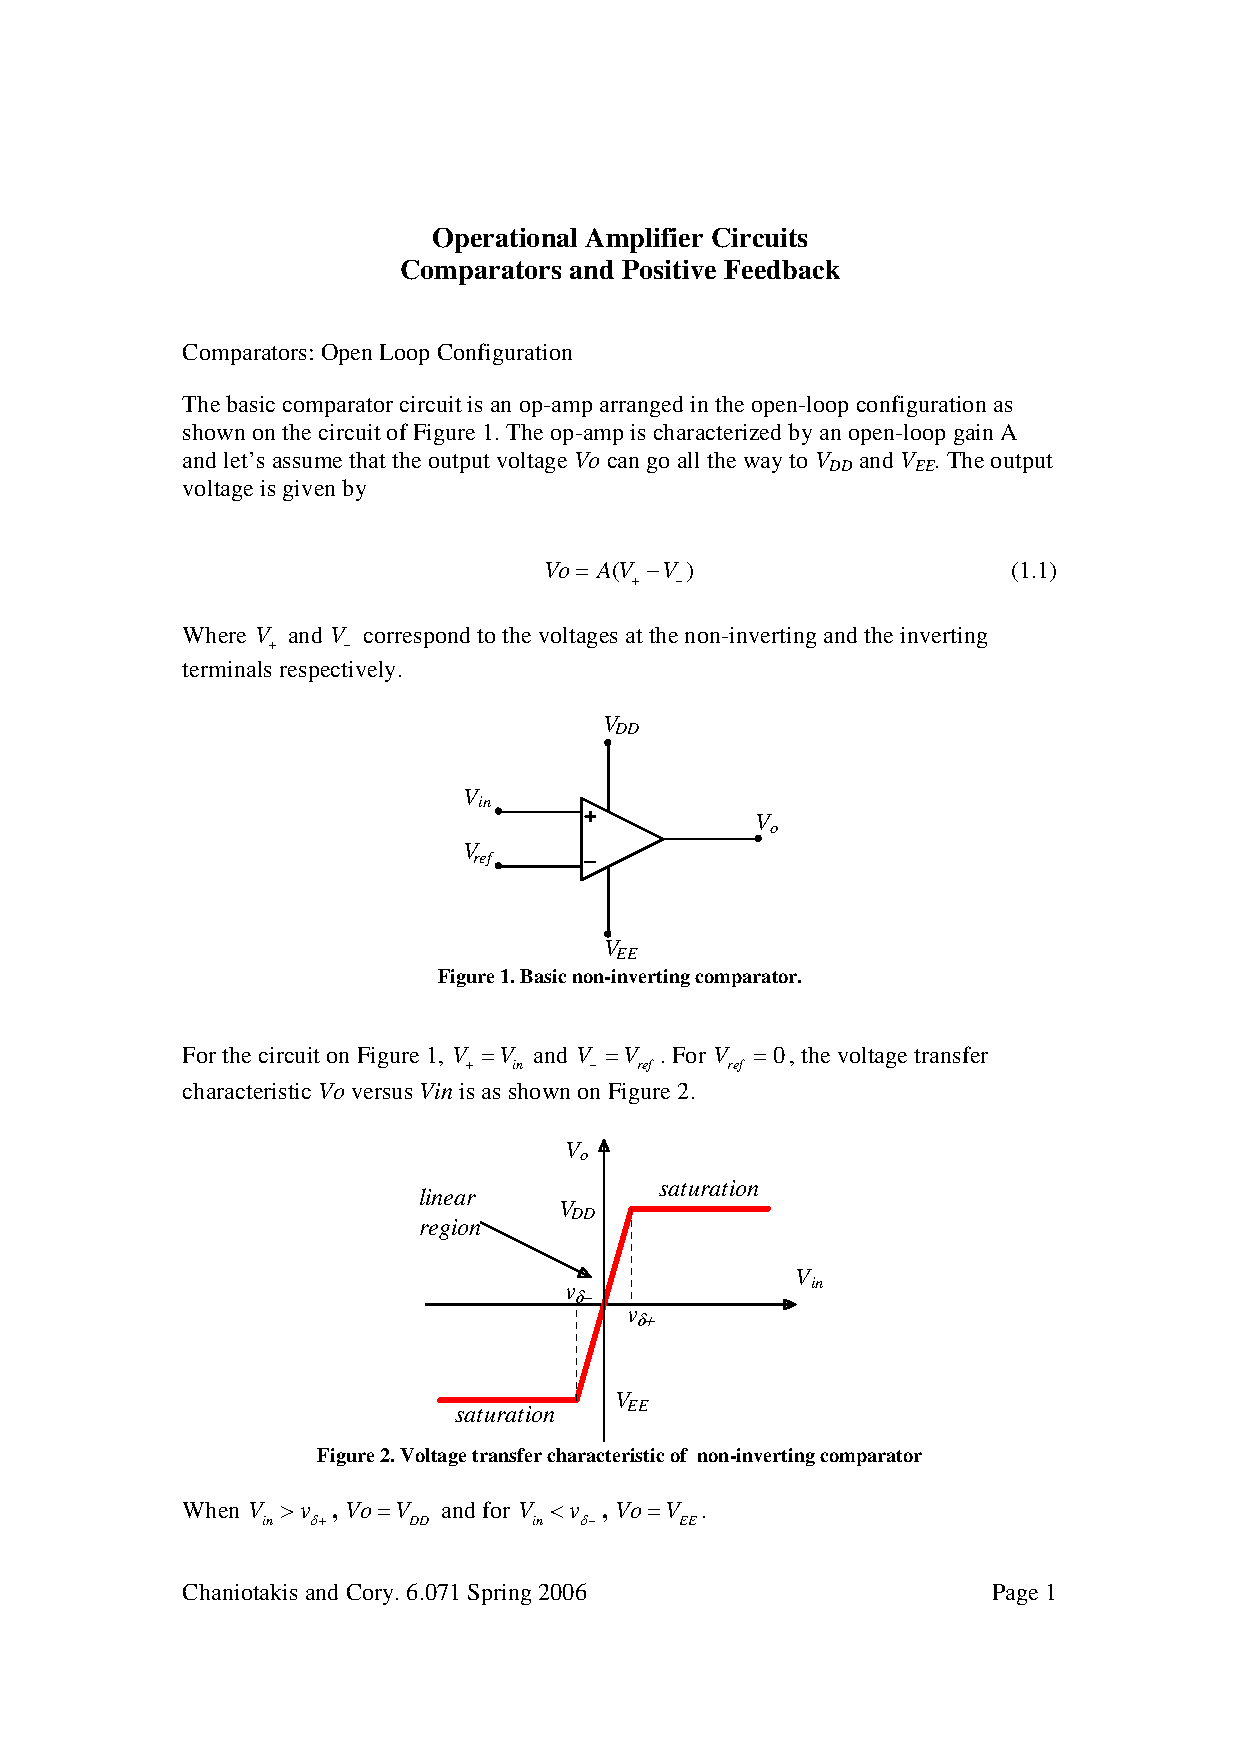
\includegraphics[page=1,width=0.8\textwidth, trim={6.9cm 5.5cm 6.9cm 19.25cm},clip]{circuits/lecture_comparator.pdf}
			\legend{Fonte: \cite{comparator-ampop-lecture}}
		\end{subfigure}
	\end{figure}

	\begin{table}[ht]
		\caption{Comportamento real de um comparador com amplificador operacional.}
		\centering
		\begin{tabular}{c c}
			\hline
			$V_{in}$ & $V_{out}$\\ \hline
			$V_{in} > V_{ref}$& $V_{CC}$\\
			$V_{in} \approx V_{ref}$& depende de $V_{\delta-}$ e $V_{\delta+}$\\
			$V_{in} < V_{ref}$& $V_{EE}$\\
			\hline
		\end{tabular}
		\label{table:comparator-behaviour}
		\caption{Fonte: Autores.}
	\end{table}

	Na primeira e terceira cláusulas da \autoref{table:comparator-behaviour}, o amplificador operacional opera na região de saturação. No entanto, seu funcionamento para entrada $V_{in} \approx V_{ref}$ polariza o semicondutor em uma região linear que depende de dois parâmetros adicionais:
	\begin{equation}
	V_{\delta+} = \frac{V_{DD}}{A}
	\end{equation}
	\begin{equation}
	V_{\delta-} = \frac{V_{EE}}{A}
	\end{equation}
	Nesse intervalo $V_{\delta-} < V_{in} < V_{\delta+}$ (ilustrado em \autoref{fig_comparator_transfer}), o comportamento da saída é diferenciado e depende do ganho de \textit{loop} aberto A, que para circuitos reais é muito grande $A=20000$. Os valores $V_{\delta-}$ e $V_{\delta+}$ então são da ordem de  $\mu$V, definindo a tensão mínima (ou máxima) da entrada para que o comparador realize uma comparação adequada. Com uma amplitude $V_{in_{AC}}$ alternada suficientemente alta, é possível tornar a curva de resposta mais íngreme melhorando o tempo de resposta do componente. A amplitude pode ser ajustada com o resistor de feedback $R_{f}$ do estágio anterior. Mesmo com essas correções, a onda comparada pode defasar um pouco na saída.

	\subsubsection*{Filtro Passa-Altas}\label{section:highpass-filter}

	Como foi observado na \autoref{plot:post-tia}, a onda recebida possui um componente $V_{DC} = L$ variável. Essa ela não tem valor fixo, então não é possível definir a tensão $V_{ref}$ para comparar. Nesse caso existe a necessidade da eliminação da componente $V_{DC} = L$.

	Para isso, pode-se utilizar um simples circuito RC de primeira ordem, que age como filtro passa-altas, esquematizado na \autoref{plot-post-highpass-filter}. Seu funcionamento se baseia no capacitor C, que em baixas frequências apresenta alta reatância, atuando como um aberto e bloqueando qualquer sinal abaixo da frequência de corte $f_{c}$. Acima dessa frequência, a reatância do capacitor é reduzida suficientemente para agir como um curto-circuito, permitindo qualquer entrada $V_{in}$ passar diretamente para saída $V_{out}$. A frequência de corte $f_{c}$ só pode ser obtida com a presença do resistor R e do capacitor C juntos, que geram a constante de tempo $\tau$. O cálculo desses valores se encontra abaixo:
	\begin{equation}
	\tau = R \cdot C
	\end{equation}
	\begin{equation}
	f_{c} = \frac{1}{2 \cdot \pi \cdot \tau}
	\end{equation}

	Ainda existe a possibilidade da fase de resposta do circuito se deslocar devido à presença do capacitor. A fórmula que calcula sua defasagem/adiantamento $\phi$ é:

	\begin{equation}
	\phi = arctan{\left(\frac{1}{2 \cdot \pi \cdot f_{op} \cdot R \cdot C}\right)}
	\end{equation}

	A \autoref{plot-post-highpass-filter} ilustra o comportamento da saída do filtro passa-altas juntamente com o esquemático do filtro passa-altas.

	\begin{figure}[h]
		\caption{\label{plot-post-highpass-filter}Saída esperada após remoção do acoplamento DC, aplicando filtro passa-alta RC de primeira ordem (à direita), com defasagem de 45$\degree$. A área hachurada representa tensão inadequada para o comparador.}
		\begin{subfigure}{.5\textwidth}
			\centering
			\begin{tikzpicture}
			\begin{axis}[
			xmin=0, xmax=25,
			ymin=-1, ymax=1,
			axis lines=middle,
			xticklabels={,,},
			ytick={-0.7, 0, 0.7},
			yticklabels={$-A_{i_{D} \cdot R_{F}}$,$0$,$A_{i_{D} \cdot R_{F}}$},
			%ylabel near ticks,
			%			ylabel style={yshift=-0.5cm},
			xlabel shift = 2 pt,
			%xlabel style={yshift=-1cm},
			xlabel={[$t$]},
			ylabel={[$V_{out}$]},
			after end axis/.code={
				\path (axis cs:0,0)
				%			node [anchor=north west,yshift=-0.075cm] {$V_{EE}$};
				node [anchor=south east,xshift=-0.2cm, yshift=-0.3cm] {$0$};
			}
			]
			\addplot[name path=f, smooth, domain=0:8*pi, color=red]{0.7*sin(deg(x/2 - pi/2))};
			\addplot[name path=axis, domain=0:8*pi]{0};
			\addplot[fill=none]
			fill between[
			of=f and axis,
			soft clip={domain=0:8*pi},
			split,
			every segment no 0/.style = {pattern=north east lines},
			every segment no 2/.style = {pattern=north east lines},
			every segment no 4/.style = {pattern=north east lines}
			];
			\end{axis}
			\end{tikzpicture}
		\end{subfigure}%
		\begin{subfigure}{.5\textwidth}
			\centering
			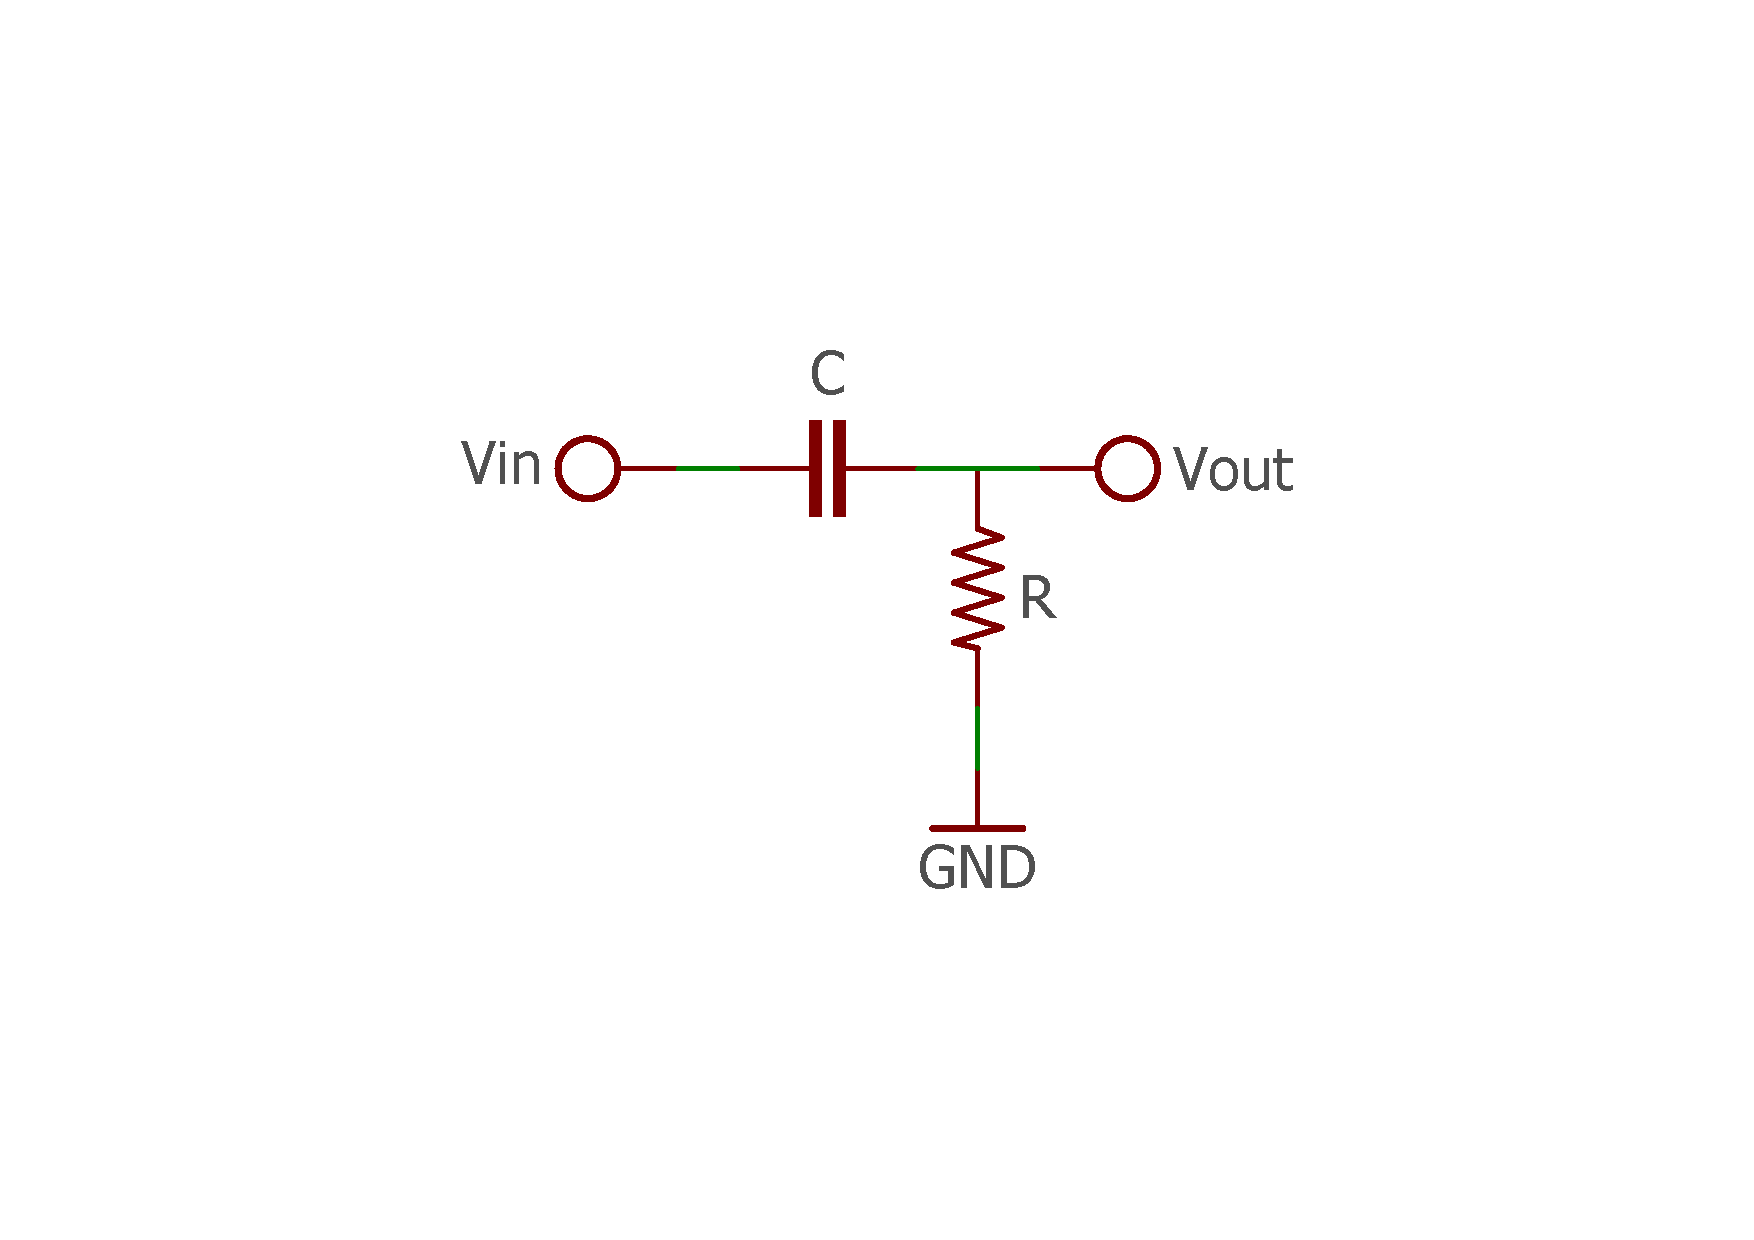
\includegraphics[width=1\textwidth, trim={3cm 0cm 3cm 3cm},clip]{circuits/highpass_filter.pdf}
		\end{subfigure}
		\legend{Fonte: Autores.}
	\end{figure}

	\subsubsection*{Acoplamento DC}\label{section:dc-bias}
	Com a aplicação do filtro passa-altas agora a onda gerada tem componente $V_{DC} = 0$ fixa - observada na parte hachurada da \autoref{plot-post-highpass-filter}, que ainda necessita correção, pois é uma tensão incompatível com o circuito.

	O funcionamento do comparador (e de qualquer amplificador operacional) depende altamente do fato de que as voltagens de entrada $V_{in}$ e $V_{ref}$ estejam dentro do intervalo de alimentação. Caso as tensões aplicadas nas entradas sejam muito altas (ou baixas), o amplificador pode operar incorretamente, ser reversamente polarizado e até ser danificado. Esses valores costumam estar presentes em \textit{datasheets} de componentes em uma tabela chamada \emph{Absolute Maximum Ratings}. Como foi decisão de projeto o fato de que o sistema de comunicação utilizaria apenas uma fonte de alimentação, essa restrição será aplicada para todos os componentes do circuito.

	Apenas uma fonte significa que o circuito terá apenas alimentação positiva disponível em seus terminais:
	\begin{equation}
	V_{in}, V_{ref} \in [V_{EE} \geq 0, V_{CC} > V_{EE}]
	\end{equation}

	Portanto, o componente não conseguirá realizar a comparação corretamente. Para resolver esse problema pode-se adicionar um acoplamento $V_{DC} = V_{ref}$ fixo, que também será utilizado na entrada de referência do comparador. E a etapa de filtro pode ser realizada juntamente com a adição de $V_{ref}$, utilizando um circuito levemente modificado.

	\begin{chart}[h]
		\caption{\label{plot-post-bias1v}Gráfico com adição de componente DC $V_{DC} = V_{ref}$ fixa e filtro passa-altas modificado.}
		\begin{subfigure}{.5\textwidth}
			\centering
			\begin{tikzpicture}
			\begin{axis}[
			xmin=0, xmax=25,
			ymin=0, ymax=2,
			axis lines=middle,
			xticklabels={,,},
			ytick={0.3, 1, 1.7},
			yticklabels={$V_{ref}-A_{i_{D} \cdot R_{F}}$,$V_{ref}$,$V_{ref}+A_{i_{D} \cdot R_{F}}$},
			%ylabel near ticks,
			%ylabel style={yshift=-0.5cm},
			xlabel shift = 2 pt,
			xlabel style={yshift=-1cm},
			xlabel={[$t$]},
			ylabel={[$V_{out}$]}
			]
			\addplot[smooth, domain=0:8*pi, color=red]{0.7*sin(deg(x/2 - pi/2)) + 1};
			\addplot[domain=0:8*pi]{1};
			\end{axis}
			\end{tikzpicture}
		\end{subfigure}
		\begin{subfigure}{.5\textwidth}
			\centering
			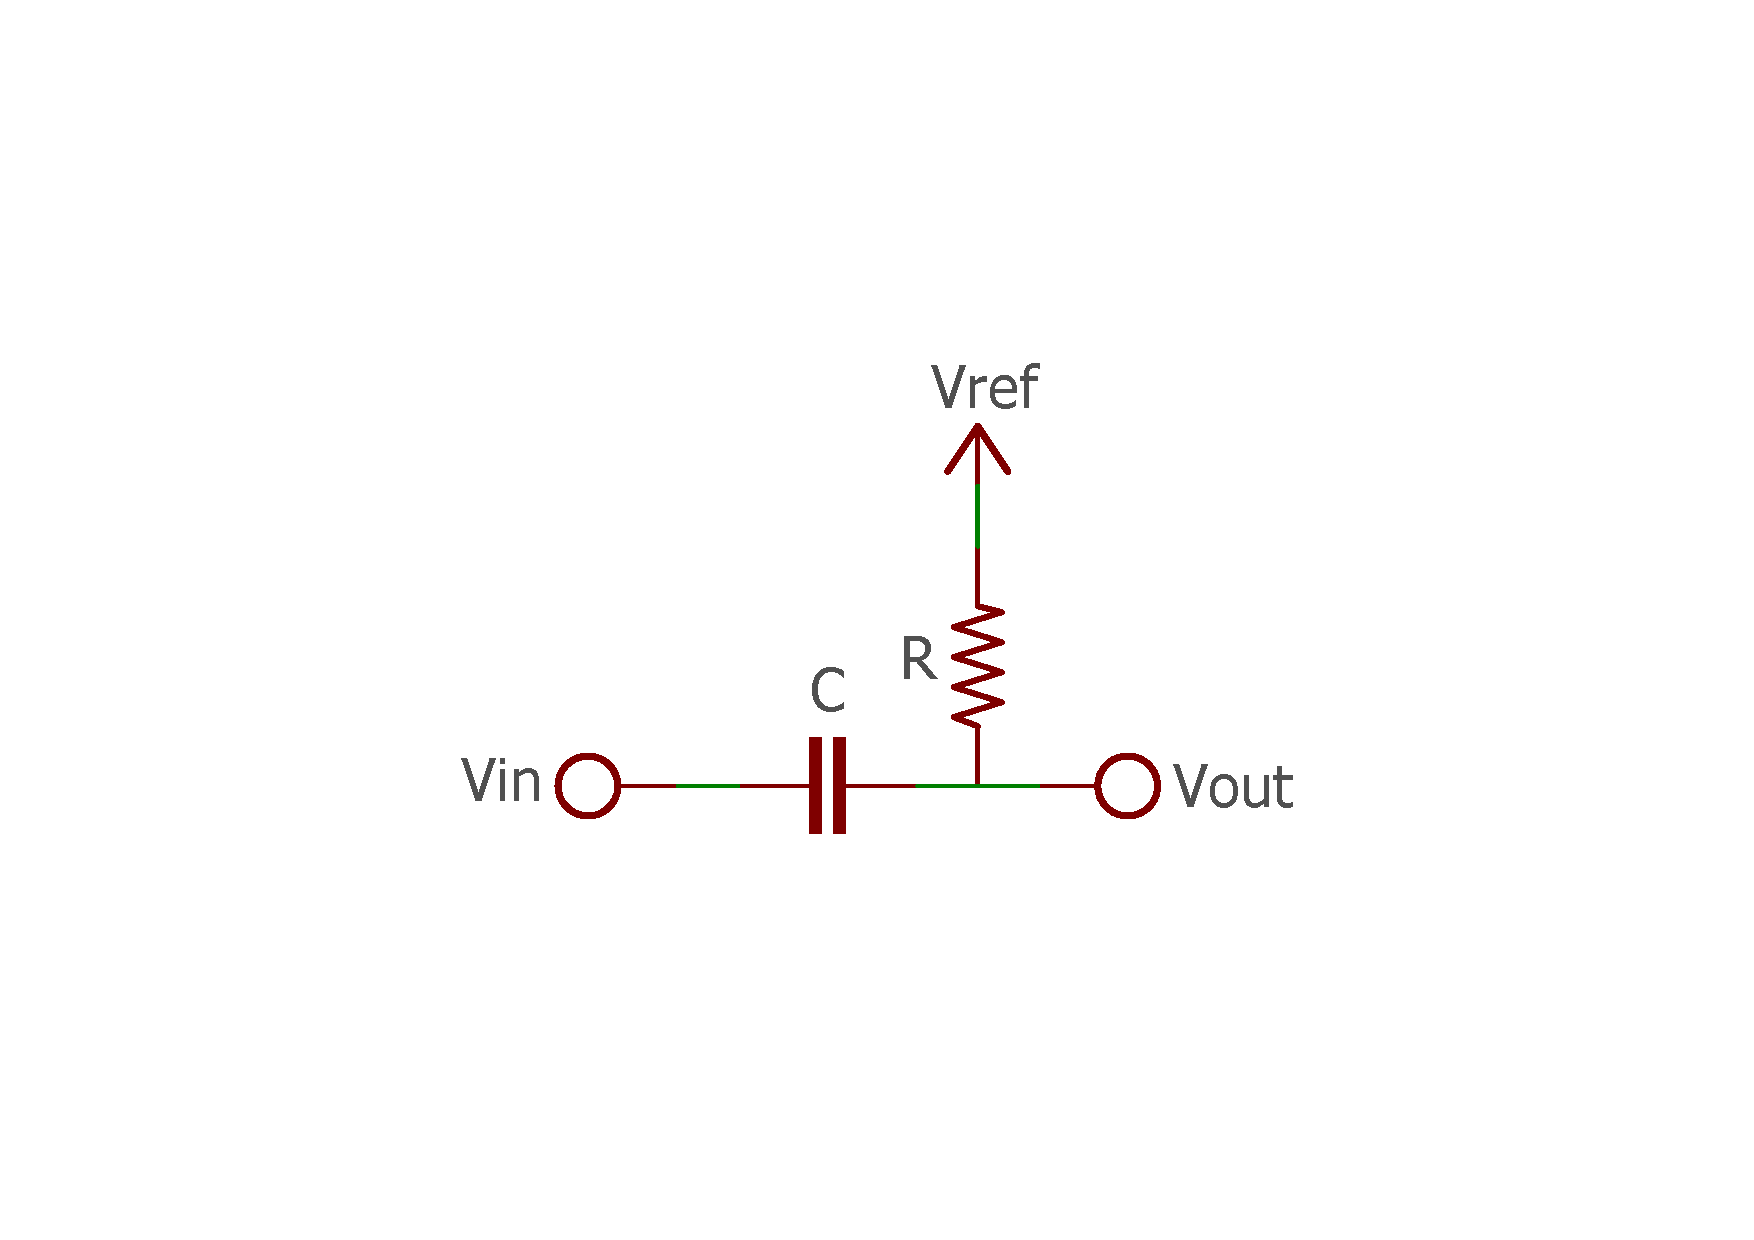
\includegraphics[width=1\textwidth, trim={3cm 0cm 3cm 3cm},clip]{circuits/highpass_filter_bias.pdf}
		\end{subfigure}
		\legend{Fonte: Autores.}
	\end{chart}

	O gráfico \ref{plot-post-bias1v} ilustra a onda modificada, agora com voltagem de referência fixa. Após todas essas etapas, é possível realizar de fato a etapa de comparação. Idealmente a onda ficaria similar ao gráfico \ref{plot-post-comparator}.

	\begin{chart}[h]
		\caption{\label{plot-post-comparator}Saída esperada após a etapa de comparação em verde.}
		\centering
		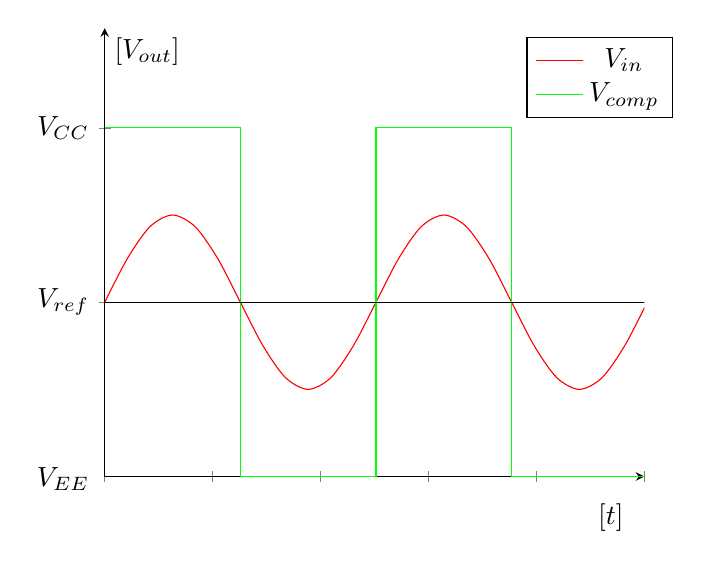
\begin{tikzpicture}
		\begin{axis}[
		xmin=0, xmax=25,
		ymin=0, ymax=1.8,
		axis y line=middle,
		axis x line=bottom,
		xticklabels={,,},
		ytick={0, 0.7, 1.4},
		yticklabels={$V_{EE}$, $V_{ref}$, $V_{CC}$},
		%ylabel near ticks,
		ylabel style={yshift=0cm, xshift=0cm},
		xlabel style={xshift=3cm, yshift=0.1cm},
		legend style={anchor=north east, xshift=0.5cm},
		xlabel={[$t$]},
		ylabel={[$V_{out}$]},
		after end axis/.code={
			\path (axis cs:0,0)
%			node [anchor=north west,yshift=-0.075cm] {$V_{EE}$};
			node [anchor=south east,xshift=-0.075cm, yshift=-0.3cm] {$V_{EE}$};
		}
		]
		\addplot[smooth, domain=0:8*pi, color=red]{0.35*sin(deg(x/2)) + 0.7}; \addlegendentry{$V_{in}$};
		\addplot[color=green] coordinates {(0, 1.4) (2*pi,1.4) (2*pi,0) (4*pi,0) (4*pi,1.4) (6*pi,1.4) (6*pi,0) (8*pi,0)}; \addlegendentry{$V_{comp}$};
		\addplot[domain=0:8*pi]{0.7};
		\end{axis}
		\end{tikzpicture}
		\legend{Fonte: Autores.}
	\end{chart}

	Com a sensibilidade ajustada de acordo, é possível que o sinal recebido seja muito semelhante (se não exatamente igual) ao enviado. Caso a saída não esteja adequada, é possível que seja necessário realizar mais um estágio de amplificação e filtração após o filtro passa-altas.

	\subsubsection*{Filtro Passa-Faixas}\label{section:band-filter}

	Com intuito de reduzir o ruído em circuitos de amplificação com amplificadores operacionais, especifica-se um modelo de circuito passa-faixas na \autoref{fig_opampdif}.

	\begin{figure}[h!]
		\caption{\label{fig_opampdif}Circuito amplificador de diferenças.}
		\centering
		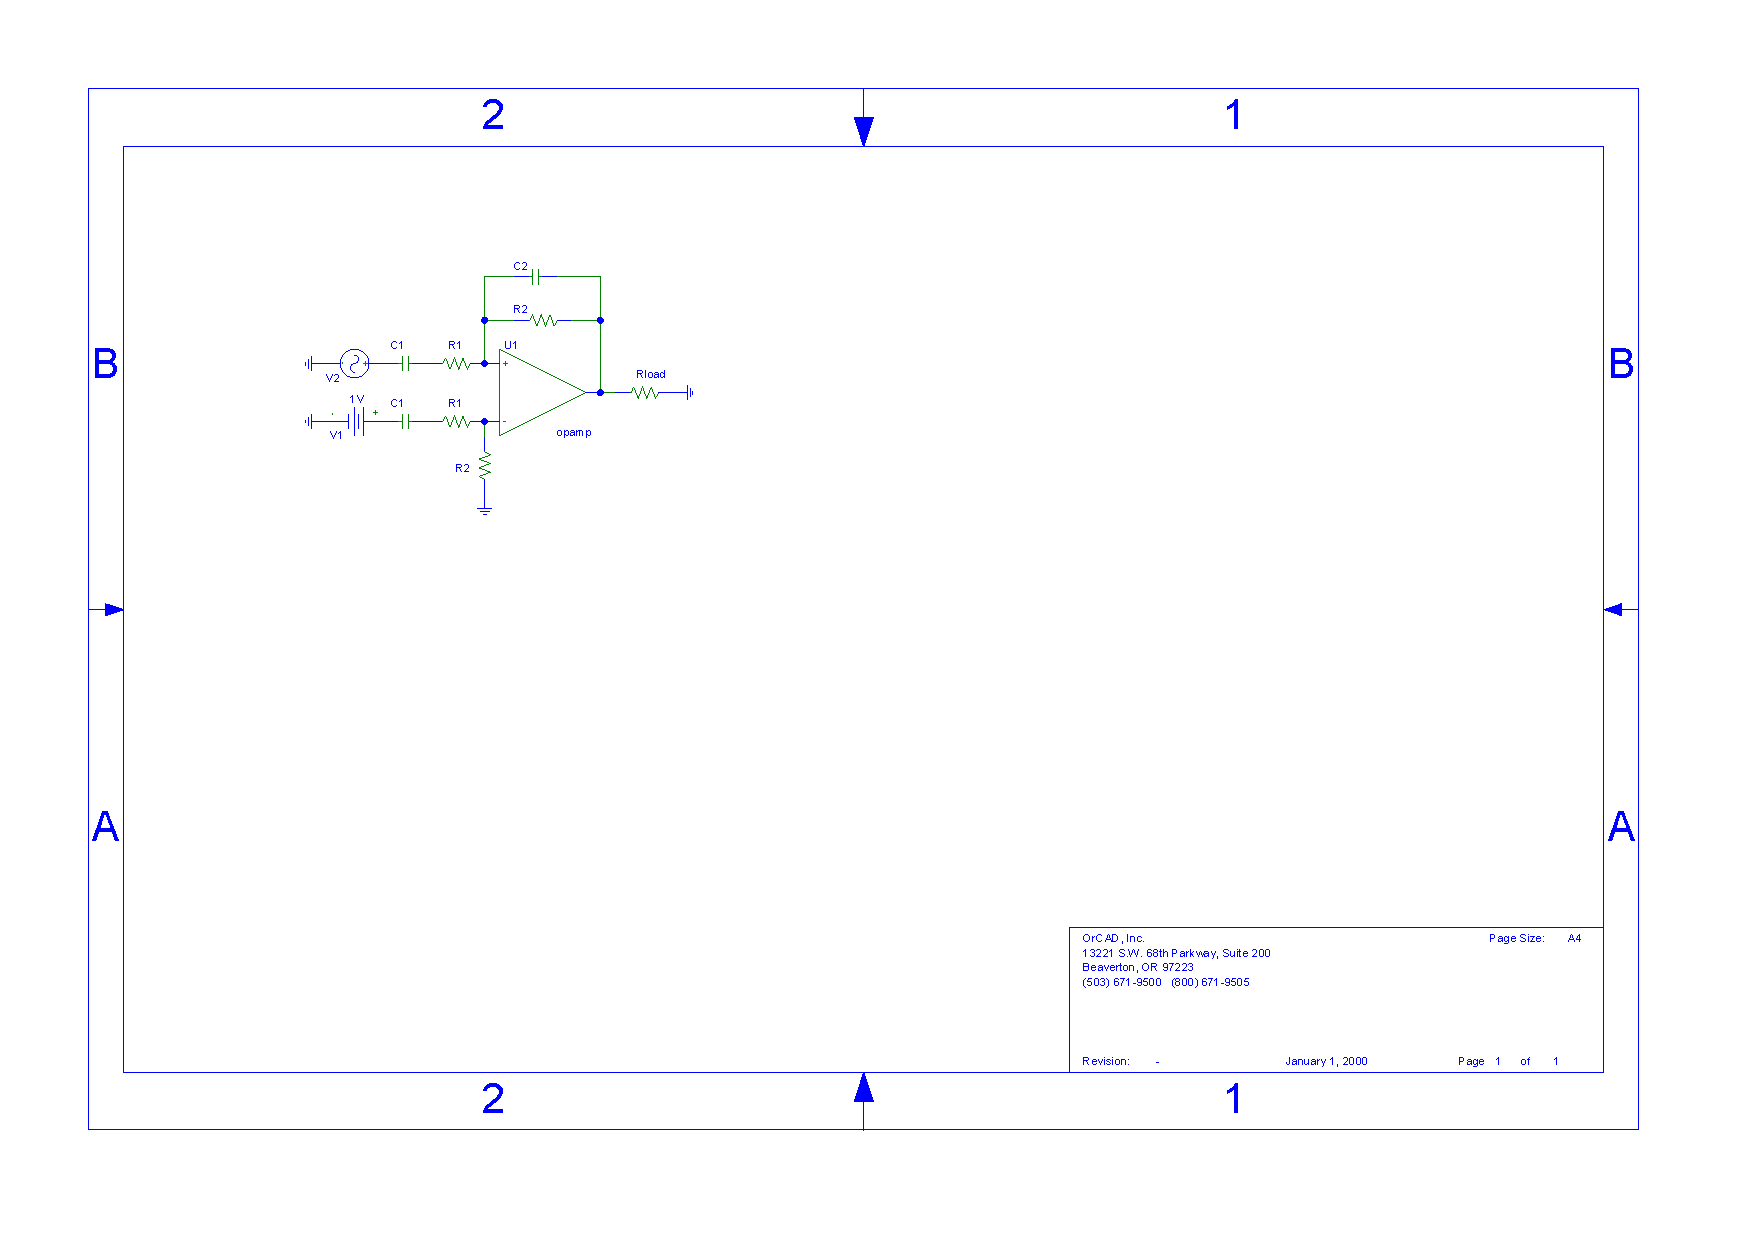
\includegraphics[width=0.6\textwidth, trim={5cm 12.29cm 17.6cm 4.3cm},clip]{circuits/opamp-dif2.pdf}
		\legend{Fonte: Autores}
	\end{figure}

	De acordo com a tabela \ref{tab_phy1} e a norma PHY II, o intervalo da frequência do \textit{clock} luminoso é de 200kHz até 120MHz. Deseja-se então  permitir a passagem dessas, limitando as frequências fora desse intervalo. Com o uso do passa-baixas e passa-altas da figura acima, pode-se realizar essa limitação adequando os resistores e capacitores do circuito.

	Deve-se levar em conta também o ganho do circuito, que é dado pela fórmula:

	\begin{equation}
	V_{out} = V_{in} \cdot \frac{R2}{R1}
	\end{equation}

	O cálculo da frequência de corte inferior do circuito é dado por:

	\begin{equation} \label{eq:1}
	f_{ci} = \frac{1}{2 \cdot \pi \cdot R1 \cdot C1}
	\end{equation}

	No caso da frequência de corte superior, pode-se realizar o cálculo utilizando a fórmula abaixo:

	\begin{equation} \label{eq:2}
	f_{ci} = \frac{1}{2 \cdot \pi \cdot R2 \cdot C2}
	\end{equation}

	O cálculo da frequência central é feita pela média geométrica das frequências calculadas em \ref{eq:1} e \ref{eq:2} acima:

	\begin{equation} \label{eq:3}
	f_{o} = \sqrt{f_{ci} \cdot f_{cs}}
	\end{equation}

	A banda de passagem do circuito é calculada pela subtração da frequência de corte superior pela inferior:

	\begin{equation} \label{eq:4}
	BW = f_{cs} - f_{ci}
	\end{equation}

	% ---
	\subsection{FPGA}\label{hard-fpga}
	% ---

	FPGA (\textit{Field-Programmable Gate Array}) é uma tecnologia que utiliza \textit{chips} de silício reprogramáveis para obter circuitos customizáveis, latência a nível de hardware e vazão muito alta. No projeto LiCy, como o fluxo de informações é muito alto (requisito de projeto de 1Gbps), é necessário realizar múltiplos processos ao mesmo tempo para lidar com os dados:

	\begin{itemize}
		\item Recebimento/Transmissão de dados
		\item Cálculo de paridade
		\item Correção de erros quando do recebimento
		\item Codificação/Decodificação de dados
	\end{itemize}

	Essa tecnologia é ideal para criar protótipos de circuitos digitais. Existe neste caso a facilidade de mudar o arranjo de componentes e vias de dados, bem como a possibilidade de simulá-los e depurá-los antes mesmo de gravar as configurações no hardware. Estes são elementos chave para a criação de um ambiente controlado e que possibilita testar as funcionalidades do produto desenvolvido, sendo um dos fatores que mais motivou a escolha dessa tecnologia neste projeto.

	O projeto de uma FPGA possui características que anteriormente estavam associadas a sistemas baseados em processadores. Uma delas é o uso de ferramentas e interfaces de alto nível, usando diagramas de bloco representando comportamentos e linguagens de descrição de hardware (na sigla em inglês, HDL), que no entanto diferem em muito de linguagens de programação como C.

	A principal vantagem do uso de uma FPGA em relação a microcontroladores está na independência das operações de processamento que, por estarem em circuitos paralelos, não precisam dividir recursos como um mesmo núcleo, por exemplo. Entretanto, o alto grau de paralelismo pode resultar em maiores desafios, como garantir o sincronismo e lidar com inconsistência de dados no nível de circuito. Ainda assim, é preferível neste projeto lidar com esses desafios para se beneficiar do ganho em latência e vazão de dados.

	% ---
	\section{Suporte ao hardware digital}\label{sec-software}
	% ---

	Esta seção explica outras escolhas feitas no aspecto de desenvolvimento de circuitos digitais do projeto.

	% ---
	\subsection{VHDL}\label{soft-vhdl}
	% ---

	VHDL, sigla do inglês para \textit{Very High Speed Integrated Circuit Hardware Description Language}, é uma linguagem de descrição de hardware. Entre suas características incluem-se uma tipagem forte, comportamento determinístico em comparação com outras linguagens de descrição de hardware como Verilog, e aplicação maior em FPGAs na área acadêmica. Por esses motivos, a curva de aprendizado pode ser mais inclinada no início, mas uma vez ultrapassada a barreira da maior rigidez no processo de compilação, a detecção de erros em código é facilitada.

	Uma linguagem de descrição de hardware tem por objetivo modelar sistemas digitais através de código. Alguns parâmetros importantes dessa modelagem são o comportamento, a estrutura e o tempo - todos cobertos por VHDL. Analogamente às linguagens de programação, VHDL possui categorias de dados, como sinais, variáveis e constantes, que servem para representar fios, registradores e outros elementos de circuitos relacionados a dados.

	Além disso, a linguagem VHDL é uma ferramenta interessante para a construção de máquinas de estado finitos. A síntese desse tipo de circuito é essencial para a implantação em hardware de algoritmos que envolvem iteração, o que é mais uma forte justificativa para a escolha desta ferramenta neste estudo. Outro fator importante levado em consideração para essa escolha foi a familiarização prévia com VHDL durante o curso, nas matérias de Laboratório, Organização e Arquitetura de Sistemas Digitais, o que auxiliou na escalada da curva de aprendizado.

	% ---
	\subsection{Quartus}\label{soft-quartus}
	% ---

	Quartus é um software de programação de dispositivos lógicos, desenvolvido pela Altera, subsidiária da Intel, que fabrica dispositivos lógicos programáveis, como as FPGAs citadas anteriormente. Algumas das vantagens dessa ferramenta são a possibilidade de sintetizar circuitos a partir de diagramas lógicos,  simular o comportamento de circuitos no tempo, controlando entradas através de \textit{testbenchs}, e uma interface relativamente simples para se programar uma FPGA.

	Dentro do contexto do estudo de sistemas digitais, os integrantes do grupo puderam se familiarizar com o software Quartus. Ademais, o fato desta ferramenta se integrar com famílias de FPGAs como Cyclone ou MAX (PLD) foi interessante, já que isto tornou possível o uso da infra-estrutura presente nos laboratórios da Universidade.
